\setcounter{tocdepth}{5}

\section{Tervezés}
\label{sec:tervezes}

\subsection{Bevezető}

Ebben a részben elsőként specifikálom a csoportos multimédia üzenetküldéssel szemben támasztott követelményeket, meghatározom a rendszer funkcionális egységeit, majd leírom, illetve összehasonlítom a rendszer megvalósításának lehetőségeit. Végül részletesen tárgyalom az általam kiválasztott megvalósítás funkcionális egységeit, a egyes részek feladatát, illetve egymással való kapcsolatát.

\subsection{A csoportos üzenetküldés}
\label{sec:group_messaging}

A csoportos üzenetküldés lényege, hogy a felhasználók egy üzenetet nem egyetlen címzettnek szeretnének elküldeni, hanem egy általuk meghatározott felhasználói csoport minden tagjának. Az üzenet típusa lehet egyszerű szöveg, de lehet bármilyen más adattípus is, mint például audiovizuális tartalom. 

Először is, a szolgáltatásban a csoportok kezelésére szükség van olyan kiegészítő funkcióra, amely a csoportok menedzselését végzi. Ez része lehet magának az üzenetküldő szolgáltatásnak, de célszerű inkább egy, az IMS-ben már meglévő, adott célra létrehozott szolgáltatást használni. Ilyen például az Ericsson fejlesztőeszközében implementált PGM (Presence, Group and Data Management - jelenlét, csoport és adatmenedzsment) szolgáltatás \cite{ericsson_pgm}.

A PGM egy értéknövelt szolgáltatás, amely lehetősége ad arra, hogy az IMS alkalmazások egyszerűen kiegészüljenek jelenlét és csoportkezelési funkciókkal. Előnye, hogy a különböző alkalmazások közös erőforrásokat használnak, ezáltal a hálózat könnyebben skálázhatóvá válik, illetve egyszerűsödik az új alkalmazások implementációja és integrációja. A jelenlét funkció lehetővé teszi személyek, alkalmazások státusz infomációinak tárolását, kezelését, valamint az infomációk publikálását mások felé.
A publikálás mellett lehetőség van feliratkozni mások jelenlét infomációira, így minden információ változásról értesülhetünk. Az információ lehet személyhez kötődő (elérhetőség, hangulat), készülékhez kötődő (technikai képesség) vagy szolgáltatáshoz kötődő (hely információ).

A PGM szolgáltatás másik része az adat és csoportmenedzsmentet ellátó funkció. Segítségével módunkban áll egy tulajdonoshoz (felhasználó vagy tetszőleges szolgáltatás) kapcsolódó címlistákat, csoportokat létrehozni, kezelni. A listák, csoportok tulajdonos specifikusak, azaz tulajdonosonként különböző információkat tartalmazhatnak. Az adatok hálózatról elérhetőek, módosíthatóak. Természetesen az adatok védettek, így azok eléréséhez megfelelő jogosultsággal kell rendelkezni. A funkció széles spektrumon felhasználható, például telefonkönyv kapcsolatok kezelésére, vagy esetemben a csoportos üzenetküldés során. 

Visszatérve a csoportos üzenetküldéshez, előfordulhat, hogy az üzenet küldésekor a címzett csoport tagjai közül néhány felhasználó éppen nem kapcsolódik a hálózathoz, azaz nem elérhető. Mivel a címzettnek szánt üzenetek nem veszhetnek el, amíg ő maga nem elérhető, így a szolgáltatásnak késleltetett üzenetkézbesítési funkciókat is el kell látnia. Utóbbi azt jelenti, hogy amíg az adott felhasználó nem elérhető, addig a neki szánt új üzeneteket átmenetileg el kell tárolni.

Az üzenetküldés magasszintű folyamata \aref{fig:group_messaging}.~ábrán látható. A küldő felhasználót \emph{A-val} jelöltem, aki a \emph{B-vel}, \emph{C-vel} és \emph{D-vel} jelölt felhasználókat tartalmazó csoportnak küld üzenetet. A \emph{B} és \emph{C} felhasználók a küldés pillanatában kapcsolódnak a hálózathoz, azaz elérhetőek, de a \emph{D} felhasználó nem. Esetében az üzenetet el kell tárolni, amely késleltetve kerül továbbításra, amikor a felhasználó elérhetővé válik.

\begin{figure}[htbp]
\center
\resizebox{9cm}{!}{
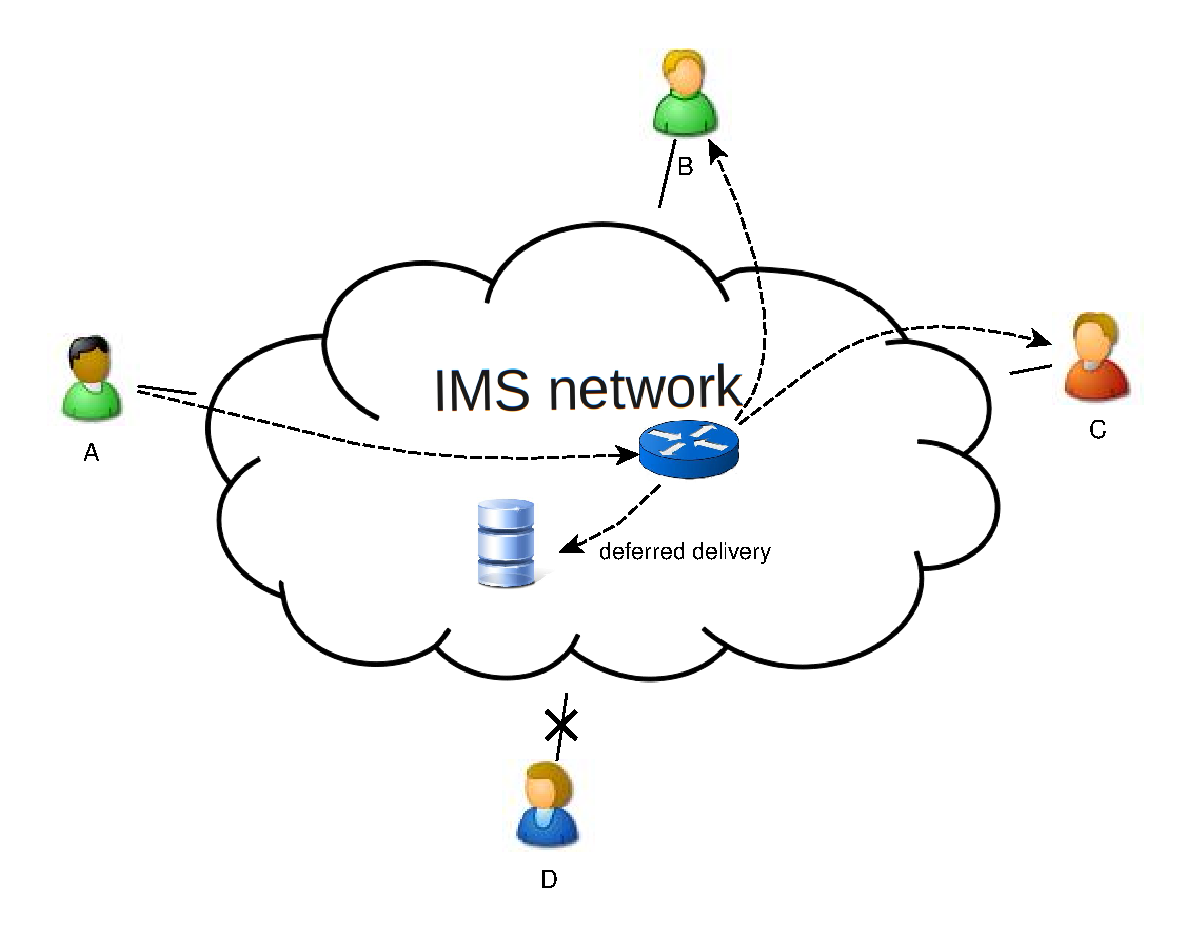
\includegraphics{img/group_messaging.eps}}
\caption{A csoportos üzenetküldés}
\label{fig:group_messaging}
\end{figure}

Hogyan valósulhat meg a késleltetett üzenettovábbítás? Kétféle módszer lehetséges:

\begin{itemize}\itemsep1pt
\item	A szolgáltatás a kézbesítetlen üzeneteket akkor továbbítja a kliensnek, amikor az regisztrál a hálózaton, azaz elérhetővé válik.
\item Amikor a felhasználó kapcsolódik a hálózathoz, nincs automatikus értesítés, hanem a felhasználó igény szerint lekérdezi az új üzeneteit.
\end{itemize} 

Az első esetben a szolgáltatás felelőssége az új üzenetekről értesíteni a felhasználót (push jelleg), amíg a második esetben a kliens alkalmazásban kell a logikát megvalósítani (pull jelleg). Véleményem szerint az üzenetküldő szolgáltatás funkciójából fakadóan az első megoldás a javasolt, mivel a szolgáltatást használó kliens oldali alkalmazások így egyszerűbbek lehetnek, amely jelentősen egyszerűsíti a kliens oldali alkalmazások fejlesztését.

A következő fejezetben megvizsgáljuk, hogy milyen lehetőségek vannak a csoportos üzenetküldés megvalósítására.

\subsection{Megvalósítási lehetőségek}

Nézzük meg, hogy az IMS használata esetén milyen lehetőségek kínálkoznak a csoportos üzenetküldés megvalósítására. A megoldási lehetőségek ismertetése során kitérek azok előnyeire, hátrányaira, illetve a felmerülő problémákra.

\subsubsection{SIP MESSAGE üzenetek használata}
\label{sec:sip_message}

Első megoldásként kézenfekvőnek tűnhet, hogy a SIP protokoll által nyújtott MESSAGE típusú üzenet törzsében küldjük el a multimédia üzenetet a címzetteknek. Ennek a megoldásnak az az előnye, hogy nem kell másik protokollt használni az üzenetek átvitelére, hanem a SIP protokoll nyújtotta funkciókat alkalmazzuk. 

A SIP MESSAGE üzenetek fejlécében a SIP protokoll szerint egyetlen címzett adható meg. Ez a csoportos üzenetküldés során erős megszorítást jelent, mivel minden címzettnek külön-külön kellene elküldeni ugyanazt a törzset tartalmazó MESSAGE üzenetet, ami jelentős redundanciához vezet. Utóbbi tény a szűk sávszélességű hozzáférési hálózatokon nem célravezető. A SIP protokoll fejlesztői felismerték ezt a problémát, és kidolgoztak egy megoldást a több címzettek rendelkező üzenetek kezelésére.
A megoldás lényege, hogy létrehoztak egy szolgáltatást, amely az üzenet címzettekhez való továbbításáért felelős. A szolgáltatást a továbbiakban URI-lista szolgáltatásnak nevezem~\cite{rfc5365}. A működés lényege, hogy a SIP MESSAGE kérés törzsét két részre bontották. Az egyik részben továbbra is a hagyományos üzenet tartalom (tartalom rész), míg a másik részben a címzettek listája kerül átvitelre (címzett lista rész). A feladó a SIP MESSAGE üzenet fejlécében a címzett mezőbe az URI-lista szolgáltatás URI-ját adja meg, majd az üzenet törzsében a tartalom részben megadja az üzenet tartalmát, a címzett lista részben pedig elhelyezi a címzetteket. A feladó az így létrehozott MESSAGE kérést a URI-lista szolgáltatásnak küldi el. A szolgáltatás, miután megkapta a kérést, a törzsben található listában szereplő minden címzettre létrehoz egy új MESSAGE kérést. Az új kérés fejlécében a feladó (From) mezőben az eredeti üzenet feladóját, míg a címzett mezőben (To) a címzett azonosítóját adja meg. A kérés törzsébe a tartalom részbe egy az egyben átmásolja az eredeti üzenet tartalmi részét, a címzett lista részt pedig bizonyos módosítások után teszi az új üzenet címzett lista részébe. Az így létrehozott kéréseket minden címzettnek elküldi. A megoldás kiküszöböli az a problémát, hogy a feladónak egyesével minden címzettre, többször kellene ugyanazt az üzenetet elküldenie. A megoldásnak viszont hátrányai is vannak. Egy ilyen hátrány, hogy a késleltetett üzenetkézbesítésre nem nyújt semmilyen megoldást. Mivel a kérések feladójának az eredeti feladó van beállítva, ezért az URI-lista szolgáltatás nem értesül a sikertelen kézbesítésről, valamint azt sem tudja, hogy a címzettek közül ki elérhető, és ki nem az. Ha egy címzett a hálózaton nem elérhető, akkor a neki küldött üzenet elvész. További problémát jelent, hogy a SIP MESSAGE kérés törzsének maximális mérete 1300 oktet\footnote{RFC 3428 - Session Initiation Protocol Extension for Instant Messaging \cite{rfc3428}}, amely tartalmazza a címzettek listáját is. A multimédia üzenet mérete rendszerint meghaladja ezt a limitet, így a tartalmat a küldő oldalon kisebb darabokra kell tördelni, a darabokat külön üzenetekben elküldeni, majd a vevő oldalon a kisebb részekből a teljes üzenetet rekonstruálni. A SIP protokoll kétféle módszert támogat MESSAGE kérések küldésére:

\begin{enumerate}\itemsep1pt
\item	Egymástól független MESSAGE kérések küldése a felek előzetes kapcsolatfelépítése nélkül.
\item Előzetes kapcsolatfelépítés (session) után a sessionben küldött MESSAGE kérések küldése. 
\end{enumerate}

Az első esetben a probléma gyökere, hogy a MESSAGE üzenettípus önmagában nem támogatja egy üzenet több darabban való átvitelét. A MESSAGE üzenet fejlécében nincs lehetőség olyan paramétert megadni, amiből a vevő egyértelműen el tudja dönteni, hogy a beérkező MESSAGE kérések közül melyik hordozza ugyanazon tartalom egy-egy darabját, és melyik nem, amiből következően rekonstruálni sem tudja azt. Utóbbi állítás abban az esetben igaz, amikor a küldő és fogadó fél között a tartalom átvitelére nem építünk fel SIP session-t (INVITE-200OK-ACK SIP tranzakció segítségével), hanem különálló SIP MESSAGE kérésekben küldjünk az egyes multimédia tartalom darabjait. 

A második esetben, amikor a tartalom darabjainak átvitele SIP session felépítése után a sessionben küldött MESSAGE kérések segítségével történik, a kérés fejlécében a \emph{Call-ID} mező értéke minden kérés esetén megegyezik a session egyedi azonosítójával, tehát a küldött kérésekre azonos. Értéke alapján meghatározható az összefüggő MESSAGE kérések halmaza, azaz azok a kérések, amelyek ugyanazon tartalom egy-egy darabját hordozzák. A kérések küldési sorrendje a kérés fejlécében a \emph{CSEQ} mező értéke szerint meghatározható, mivel a \emph{CSEQ} mező értéke a küldési sorrend szerint növekszik. 

Az említett két eset közül az első megoldási javaslat az említett problémák miatt nem alkalmas egy nagyobb multimédia üzenet több darabban való átvitelére, mivel a vételi oldal nem képes rekonstruálni az eredetileg küldött multimédia üzenetet. A második megvalósítás, azaz a SIP session-t használó megoldás alkalmas lehet a nagyobb multimédia tartalom részekben történő átvitelére, hátránya viszont az, hogy minden egyes címzettel külön-külön fel kell építeni egy SIP sessiont, amely sok címzett esetén rengeteg kapcsolatot igényel. Utóbbi problémára megoldást jelenthet, ha a küldő felhasználó nem a címzettekkel hoz létre külön-külön egy-egy session-t, hanem egy, az IMS hálózatban lévő alkalmazás szerveren futó szolgáltatással. A multimédia tartalom a kliens és a szerver között egyszer kerülne átvitelre, amely jelentősen csökkenti a szükséges kapcsolatok számát. A tartalom átvitele során az URI-lista szolgáltatáshoz hasonlóan a kliens egy további MESSAGE kérés törzsében elküldené a szerver oldali szolgáltatásnak a címzettek listáját, így a szolgáltatás feladata lenne a multimédia üzenet címzetteknek való kézbesítése. Az említett szolgáltatás megoldást jelentene a késleltetett üzenetkézbesítésre is. További hátrány a MESSAGE kérések törzsének erősen limitált mérete, amely egy nagyobb méretű multimédia tartalom esetén jelentősen megnöveli a MESSAGE kérések számát, amely az átvitel hatékonysága, sebessége szempontjából nem előnyös.

\subsubsection{Több címzettel rendelkező üzenetek használata}
\label{sec:mr_message}

Ebben a pontban leírt megoldás abban tér el \aref{sec:sip_message}.~fejezetben leírt megoldáshoz képest, hogy az üzenet fejlécben lehetőség van több címzettet megadni. A folytatásban az ilyen típusú üzenetet több címzettel rendelkező, azaz MR (Multi Recipient) üzenetnek fogom nevezni. A több címzett megadásának a lehetősége jelentős előnyt jelent az alap SIP MESSAGE-et használó megoldáshoz képest. Először is, a feladónak elég csak egyszer elküldeni az üzenetet a CSCF felé, és nem annyiszor, ahány címzettje van az üzenetnek. Ez jelentősen lecsökkenti a hálózati erőforrások használatát. Másodszor, mivel a címzettek az MR üzenet fejlécében helyezkednek el, így az erre alkalmas hálózati szerverek a fejléc adatokat felhasználva képesek az üzeneteket hatékonyan eljuttatni az összes címzettnek anélkül, hogy az üzenet törzsét meg kellene vizsgálniuk. Tegyük fel, hogy a feladó hálózatában lévő S-CSCF, miután megkapja feladótól az MR üzenetet, annak minden címzettjére meghatározza az adott címzett felé vezető következő állomást (next hop CSCF), ahová továbbítani kell azt. Abban az esetben, ha kettő vagy több címzett esetén ugyanaz a next hop, akkor az S-CSCF abba az irányba MR üzenetként küldi tovább az üzenetet. Ha minden címzett next hop CSCF-je különbözik egymástól, akkor a szerver az egyes next hop-oknak hagyományos üzenetben küldi el annak egy-egy másolatát. Mivel a hálózatban található összes CSCF hasonlóan viselkedik, mint a feladót kiszolgáló S-CSCF, ezzel a módszerrel két szerver között ugyanaz az üzenet pontosan egyszer kerül átvitelre. Az üzenet terjedésének folyamatát \aref{fig:mrflow}.~ábrán követhetjük nyomon. Jól látható, hogy ezzel a módszerrel minden linken kizárólag egyszer küldjük át ugyanazt az üzenetet, ellentétben az aktuális IMS javaslattal, miszerint több címzett esetén egy linken többször kellene átküldeni ugyanazt az üzenetet (Például a III-as, IV-es és V-ös linken). Abban az esetben, ha egy olyan CSCF vesz egy MR üzenetet, amely nem képes MR üzeneteket kezelni, akkor a küldő CSCF felé hibaüzenetet küld. Ilyenkor a küldő CSCF újra elküldi az üzenetet hagyományos SIP üzenetként, minden címzettre külön-külön. 

\begin{figure}[htbp]
\center
\resizebox{10cm}{!}{
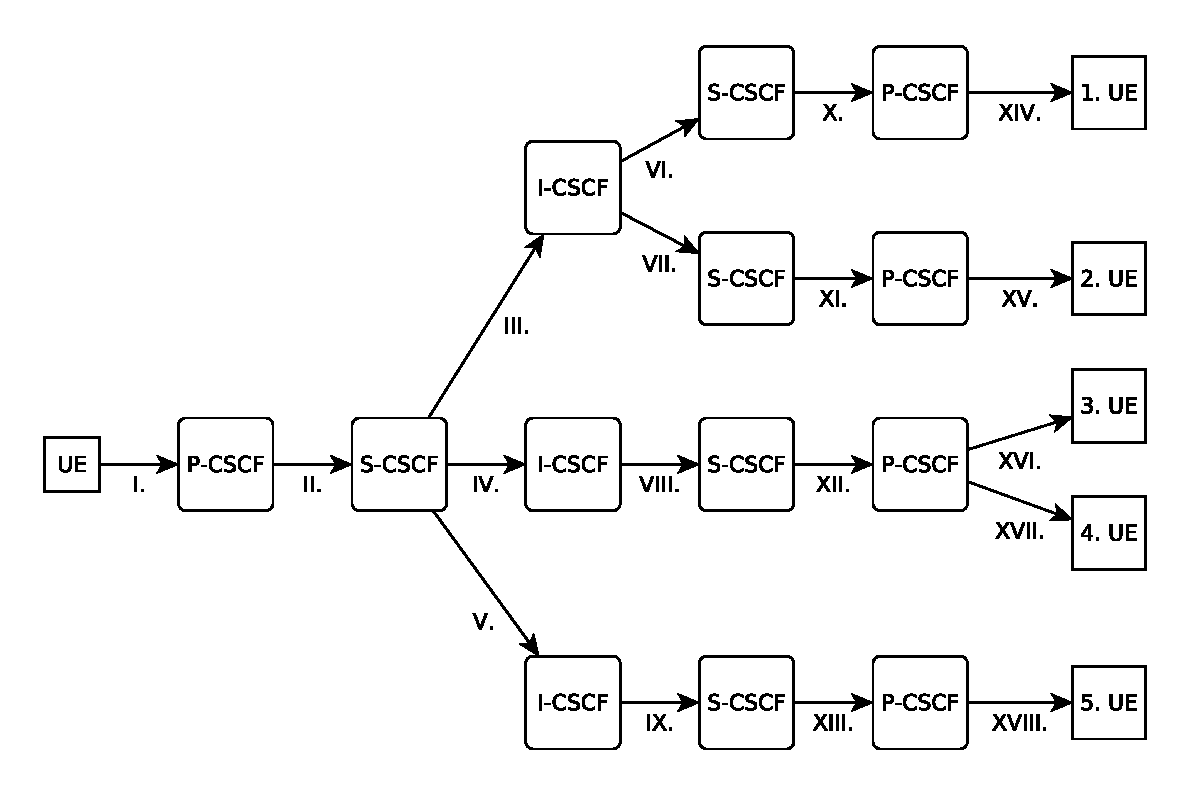
\includegraphics{img/MR-flow.eps}}
\caption{Az MR üzenetküldés folyamata}
\label{fig:mrflow}
\end{figure}

Mivel egy multimédia üzenet viszonylag nagy méretű is lehet, nagy valószínűséggel nem fér bele egyetlen MR üzenet törzsébe. Utóbbi probléma abból ered, hogy az IP hálózatokban maximalizálva van a hálózatba küldhető csomag mérete (MTU - Maximum Transmission Unit). Hasonlóan a SIP MESSAGE üzeneteket használó megoldáshoz, itt is darabolni kellene a multimédia üzenetet több kisebb csomagra. Mivel az MR csomagok akár különböző útvonalon is eljuthatnak a címzetthez, a vételi oldalon a csomagok eredeti sorrendjének visszaállíthatónak kell lennie. Amennyiben az MR üzenet fejlécében lehetőség lenne elhelyezni olyan mezőket, amelyek a helyes sorrend visszaállítását szolgálják, akkor a megoldás jelentősen jobb lenne, mint a SIP MESSAGE-et használó megvalósítás. Itt is általános feladatként jelentkezik a késleltett üzenetkézbesítés problémája, ami egy köztes alkalmazás szerver használatával megvalósítható lenne.

A vételi oldalon a kliensek, miután megkapták az MR kéréseket, nyugtázzák azokat. A cél itt is az, hogy a nyugták küldéséből eredő, a feladó és az őt kiszolgáló S-CSCF közötti linken folyó üzenetforgalmat minél jobban lecsökkentsük anélkül, hogy az IMS komponensek viselkedését alapvetően megváltoztatnánk. Ha a feladót kiszolgáló S-CSCF nem kompatibilis az MR üzenetekkel, akkor minden egyes nyugtát a hagyományos módon, egyesével továbbít a feladónak. Abban az esetben viszont, amikor az említett S-CSCF képes kezelni az MR üzeneteket, a hozzá beérkező, azonos típusú nyugtákra -- pl. 200 OK -- adott időtartamig vár, majd a nyugtákból összeállít egy MR választ, és csak ezt küldi el a feladónak, amivel jelentősen csökkenti a kérdéses link forgalmát.

\subsubsection{Üzenet továbbítása MSRP protokollal}
\label{sec:msrp_message}

Ez a megoldási javaslat a multimédia üzenetek felhasználók közötti átvitelére az MSRP (Message Session Relay Protocol) protokollt használja. Az MSRP -- a SIP-hez vagy a HTTP-hez hasonlóan -- egy szöveges, alkalmazás rétegbeli protokoll. A protokoll kapcsolat orientált adatátvitelt (session mode) tesz lehetővé, aminek számos előnye van a különálló, független üzenetcsomagok küldéséhez képest (paging mode).
Ezen előnyök közé tartozik, hogy a kommunikációs felek explicit felépítenek egymás között egy kommunikációs csatornát az üzenet csomagok átvitelére. A kapcsolat léte magában foglalja az összefüggő üzenet csomagok biztonságos, sorrendhelyes átvitelét, valamint a garantált kézbesítést is. Minden MSRP üzenet vagy egy kérés, vagy egy válasz. Az üzenetek fejlécből és törzsből állnak. A fejlécben az MSRP kapcsolatot, illetve a törzsben lévő -- szöveges vagy bináris -- tartalmat leíró információk találhatóak. Az MSRP kapcsolat felépítése SIP és SDP (Session Description Protocol) protokoll~\cite{rfc4566} segítségével történik. Az MSRP csomagok felépítésének leírása \aref{sec:msrp_chunks}.~fejezetben található. A protokollról részletesebben az~\cite{rfc4975} irodalomban olvashat. Az SDP protokoll egy olyan szabályegyüttes, amely a multimédiás tartalmakat továbbító kapcsolatok paramétereit írja le. Ilyen paraméter többek között a kapcsolat sávszélessége, a kapcsolaton átvitelre kerülő multimédiát leíró információk, az átviteli protokoll, a kommunikációs IP cím és port, stb. A kapcsolatot felépítő kommunikációs felek az SDP protokoll alapján leírják a rájuk jellemző paramétereket, majd SIP protokoll segítségével ,,megbeszélik'' egymással a felépíteni kívánt kapcsolatokat, azaz megoszják egymás között az SDP protokollal megadott paramétereket. 

Mivel a címzettek csoportjában lehet olyan felhasználó, aki az üzenet küldésének pillanatában nem elérhető, így a késletetett kézbesítés problémája ebben az esetben is felmerül. Utóbbi problémára itt is megoldást nyújt az, ha a kliensek közé egy alkalmazás szervert helyezünk el, amely többek között a késletetett üzenet kézbesítését is végzi. A köztes szerver használata a hálózati forgalmat is csökkenti, mivel a feladó és a szerver közötti, jellemzően alacsony sávszélességű (pl. rádiós) linken csak egyszer kerül átvitelre a -- gyakran nagy méretű -- multimédia üzenetet, szemben azzal az esettel, amikor a feladó minden címzettre külön-külön elküldi azt. Miután sikeresen átvitelre került a multimédia üzenet, a feladónak a címzettek listáját valamilyen módon, például egy SIP MESSAGE üzenet törzsében kézbesíteni kell a szerver felé. Mivel ez a lista jellemzően rövid szöveges üzenet, így belefér egyetlen SIP MESSAGE üzenetbe. A megoldás hátránya az MSRP kapcsolat felépítésének költsége, ami viszont a kapcsolat tényéből fakadó, már fentebb említett előnyökhöz képest elhanyagolható.

\medskip

A dolgozatban a szolgáltatás fejlesztése során a fentebb leírt megoldások közül a legutolsó, MSRP protokollt használó megoldás használata mellett döntöttem. A SIP MESSAGE üzenetek használata nem célszerű \aref{sec:sip_message}.~fejezetben leírt hátrányok miatt. \Aref{sec:mr_message}.~fejezetben tárgyalt MR üzenetet használó csoportos üzenetküldési megoldás jelenleg csak ajánlás formájában létezik, bárminemű szabványosítási eljárás jelenleg nincs folyamatban a témával kapcsolatban. Az MSRP protokollal való megvalósítás előnye a többi megoldási javaslattal szemben, hogy -- az IMS-ben jelen lévő --szabványosított eszközök használatára épít, illetve az adatátvitel kapcsolatorientált jellege következtében megbízható üzenetküldés valósítható meg. 

\subsection{Funkcionális terv}

A rendszer alapvetően a klasszikus kliens-szerver architektúrát valósítja meg. A kliensek azok, akik létrehozzák a multimédia üzeneteket, majd a szerver közvetítésével elküldik azt más kliensek egy meghatározott csoportjának. A szerver adatbázisban tárolja a multimédia üzenethez tartozó adatokat, mint például a feladó neve, SIP azonosítója, a címzettek nevei, a multimédia tartalom, stb. A küldő kliens az átvitel sikerességéről folyamatos értesítést kap a szervertől. A szerver, miután sikeresen megkapta az új üzenetet, az online címzetteknek -- egy SIP MESSAGE üzenet törzsében -- azonnal értesítést küld erről. Az említett üzenet törzsének részletes ismertetése a \aref{sec:sip_message} fejezetben található. Egy felhasználó, amikor az új üzenetről értesítést kap a szervertől, a tényleges multimédia üzenetről kapott leíró információk alapján eldöntheti, hogy érdekli-e őt az üzenet, vagy sem. Ilyen leíró információ az üzenet feladójának adatai, az üzenet tárgya, valamint az üzenet tartalmának típusa, úgy mint kép, hang vagy videó, a tartalom mérete, illetve a küldés dátuma. A kapott információk alapján a címzett eldöntheti, hogy érdekli őt az üzenet tényleges multimédia tartalma vagy sem, és ezáltal a döntésnek megfelelő akciót végrehajtsa (azaz megtekintse a multimédia üzenetet vagy sem). 

A rendszer magasszintű modelljét \aref{fig:model}.~ábra szemlélteti.

\begin{figure}[htbp]
\center
\resizebox{12.5cm}{!}{
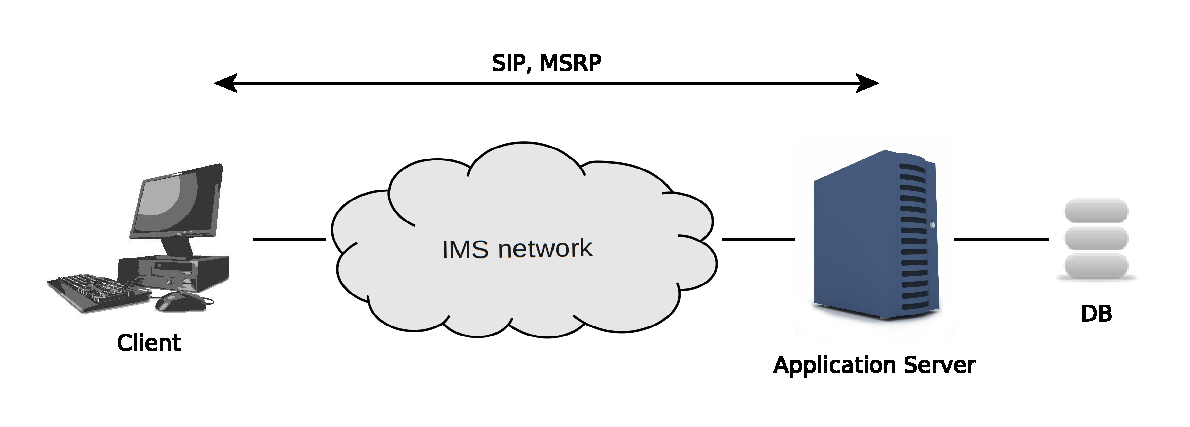
\includegraphics{img/system_MSRP_black_2.eps}}
\caption{A rendszer magasszintű modellje}
\label{fig:model}
\end{figure}

A rendszer az alábbi részekből épül fel:
\begin{mydescription}
\item[Kliens PC:] A felhasználó ezen keresztül éri el a szolgáltatást.
\item[Alkalmazás szerver:] Az üzenet fogadását és a címzetteknek való kézbesítést valósítja meg.
\item[Adatbázis szerver:] Az üzenethez tartozó adatok tényleges tárolását végzi.
\end{mydescription}

A következő fejezetekben az egyes elemek funkciójának részletes tárgyalása következik.

\subsubsection{Kliens}
\label{sec:kliens_pc}

A felhasználó ezen keresztül éri el az IMS hálózatot, azaz magát az üzenetküldő szolgáltatást is, ebből fakadóan a kliens eszköznek rendelkeznie kell hálózati kapcsolattal.

A felhasználó multimédia üzenetet küldhet más, általa ismert felhasználók csoportjának. Az elküldendő multimédia üzenet többféleképpen állhat a kliens rendelkezésére. Egyik lehetséges opció, hogy az elküldenő üzenethez tartozó multimédia tartalom már a felhasználó rendelkezésére áll kép, hang vagy videó fájl formájában. Ebben az esetben a küldő kliens fájlrendszeren való tallózással választhatja ki a multimédia tartalmat. A tartalom létrehozásának egy másik lehetséges módja, hogy a felhasználó a számítógépéhez kapcsolódó audiovizuális eszközökkel (mikrofon és kamera) maga készíti el a multimédia üzenethez a multimédia felvételt. Miután az elküldendő multimédia üzenethez a tartalom a felhasználó rendelkezésére áll, valamilyen módon el kell küldeni a szerver oldalnak. A tartalom kliens-szerver közötti átvitele MSRP protokollal történik.

Az üzenetküldés folyamatát \aref{fig:sending_proc}.~ábrán láthatjuk. A folyamat első lépéseként a küldő kliens és a szerver között fel kell építeni egy MSRP kapcsolatot, amelyen keresztül a multimédia üzenet átvitele történik. Egy MSRP kapcsolat minden esetben egy kliens és a szerver között épül fel, két kliens közvetlenül egymáshoz soha nem csatlakozik. Amikor az MSRP kapcsolat sikeresen felépült, a feladó ezen kapcsolaton keresztül MSRP csomagok\footnote{Az MSRP csomag felépítése \aref{sec:msrp_chunks}.~fejezetben található} formájában továbbítja a multimédia üzenetet a szervernek. A szerver minden MSRP csomag vételét nyugtázza a küldő kliens felé. Miután a teljes üzenet sikeresen megérkezett a szerver oldalra, kliens a folyamat következő lépéseként egy SIP MESSAGE típusú üzenet törzsében elküldi a szervernek a címzettek listáját, illetve opcionálisan egyéb, az elküldött multimédia üzenetre jellemző információt. A címzett lista, illetve a kiegészítő információk a MESSAGE kérés törzsében, XML (Extensible Markup Language) formátumban kerülnek átvitelre. Mivel az említett XML rövid, így az belefér egyetlen SIP MESSAGE üzenetbe. A szerver az XML-t tartalmazó üzenet sikeres vétele után a multimédia tartalommal együtt adatbázisban eltárolja azt, majd nyugtázza a vételt a feladó felé. A küldés befejezéseként a kliens bontja az MSRP kapcsolatot a szerverrel.

\begin{figure}[htbp]
\center
\resizebox{10cm}{!}{
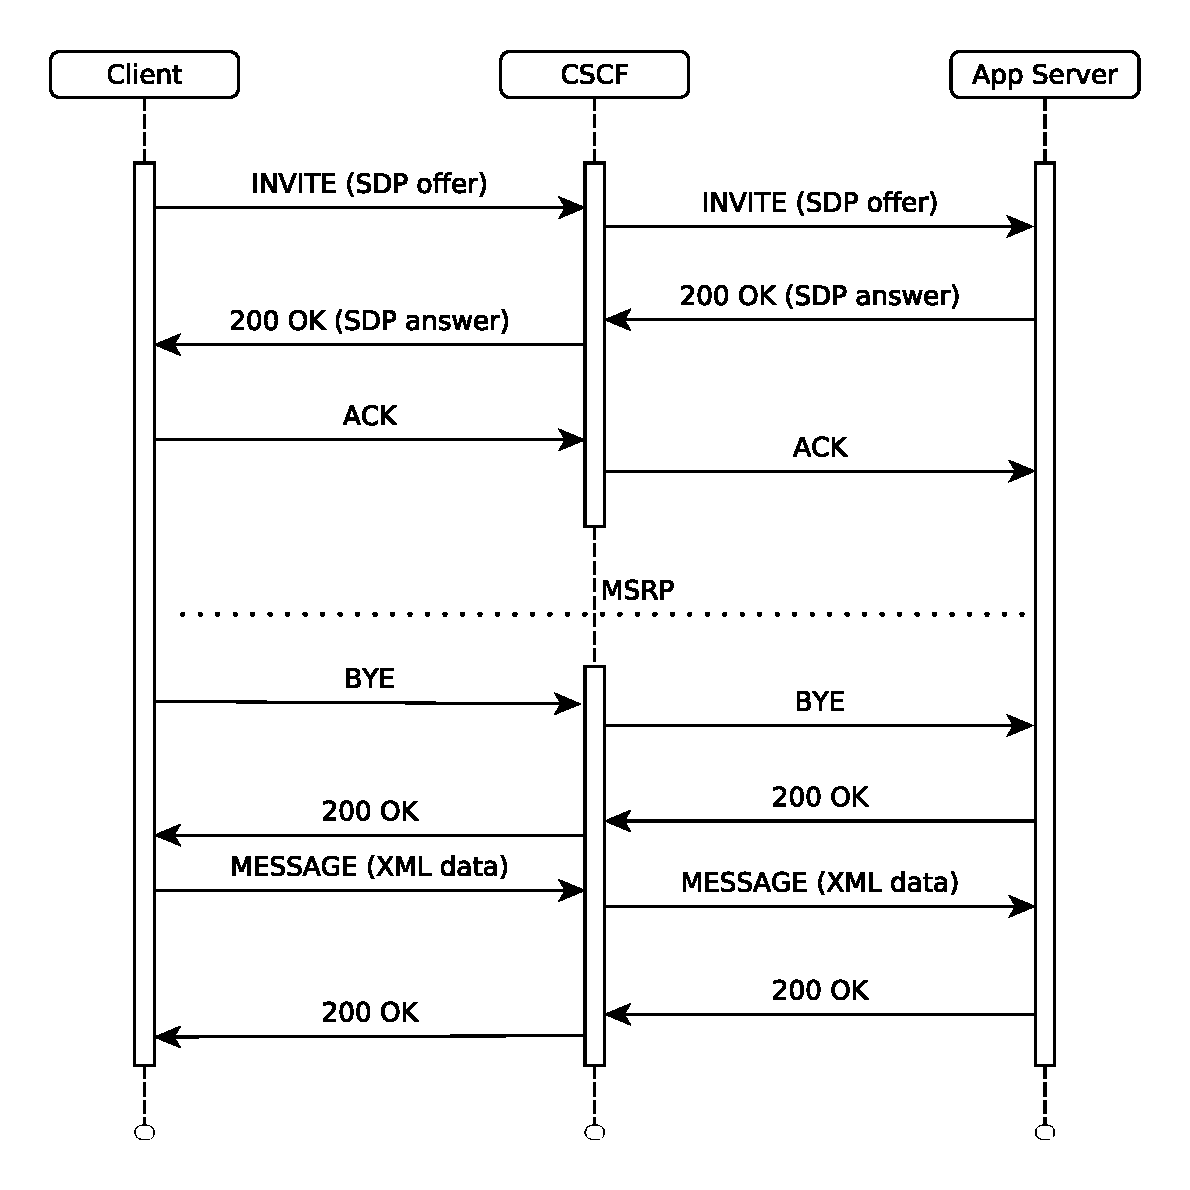
\includegraphics{img/sending_procedure.eps}}
\caption{Az üzenetküldés folyamata}
\label{fig:sending_proc}
\end{figure}

A kliens oldalon a multimédia üzenet vétele is több lépésben zajlik (\ref{fig:receiving_proc}.~ábra). Amikor a szerver új multimédia üzenetet kap, akkor a szerver első lépésként egy SIP MESSAGE üzenetben értesíti erről a címzettek közül azokat a felhasználókat, amelyek a regisztrált felhasználók listájában szerepelnek, azaz elérhetőek. Utóbbi üzenet törzse szintén XML formátumban tartalmazza a multimédia üzenetekre jellemző adatokat. Második lépésként a felhasználó az XML-ben kapott információk alapján eldönti, hogy kiváncsi egy adott multimédia üzenetre, vagy sem. Amennyiben érdekli maga a multimédia tartalom is, felépít egy MSRP kapcsolatot a szerver oldallal, amelyen keresztül ,,letölti'' magát a tartalmat. A felhasználó dönthet úgy, hogy jelenleg nem kiváncsi az adott multimédia üzenetre. Utóbbi esetben nincs semmilyen további kommunikáció a kliens és a szerver között. A felhasználónak lehetősége nyílik egy adott multimédia üzenet tartalom átvitele nélküli törlésére is, ilyenkor szintén SIP MESSAGE üzenetben értesíti erről a szervert. Utóbbi esetben a a szerver a multimédia üzenet felhasználóhoz tartozó bejegyzésének kézbesítési státuszát ,,törölt''-re állítja. A szerver a törölt státuszú bejegyzéseket periodikusan törli az adatbázisból.

\begin{figure}[htbp]
\center
\resizebox{10cm}{!}{
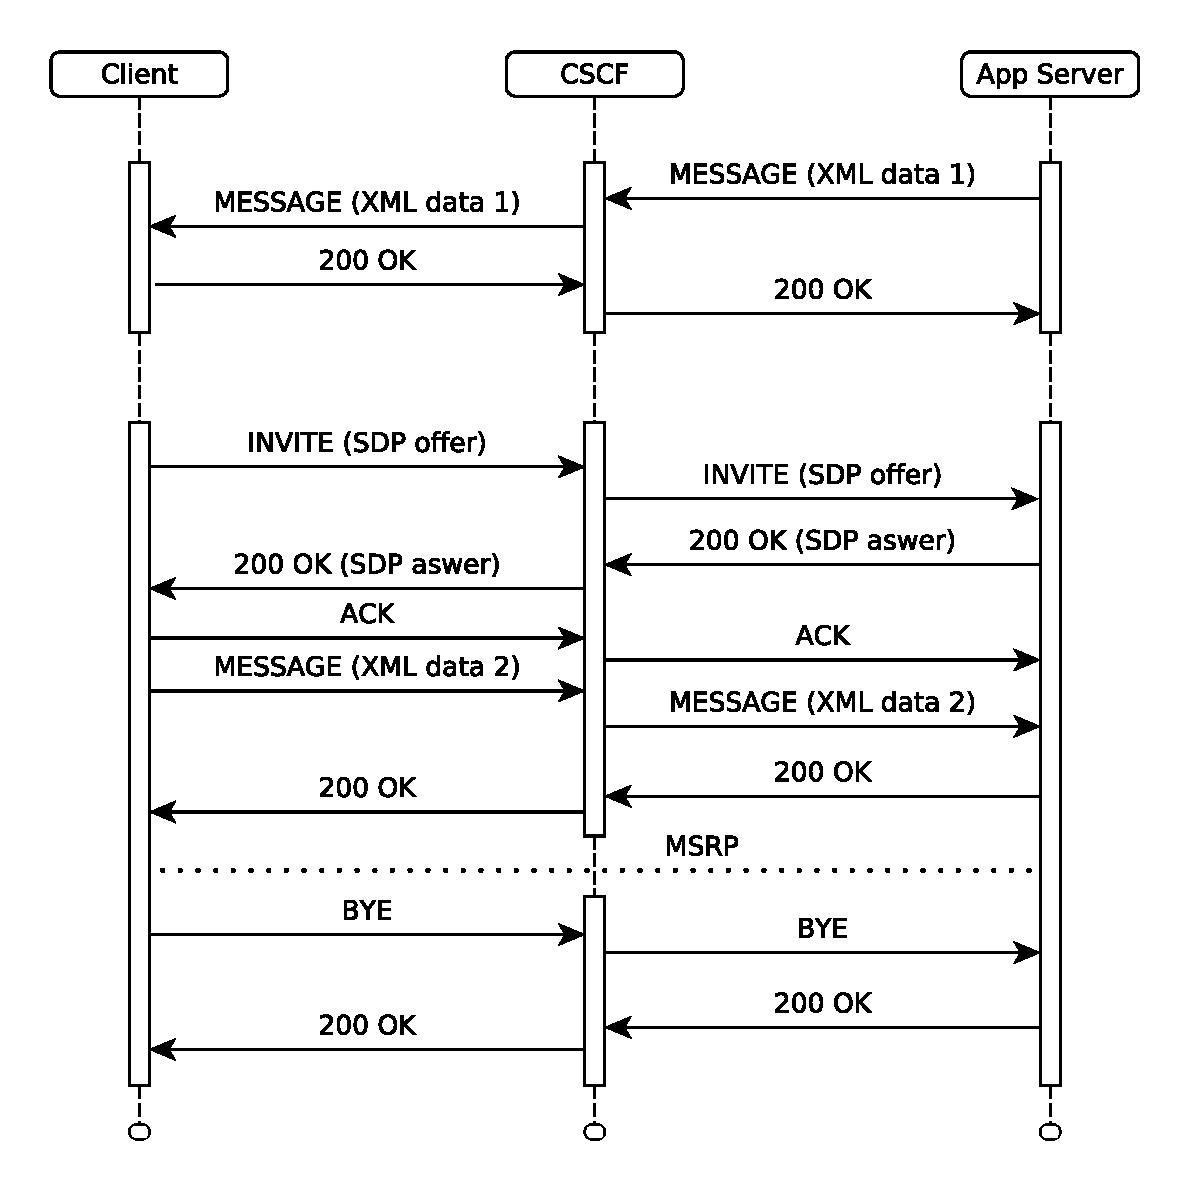
\includegraphics{img/receiving_procedure.eps}}
\caption{Az üzenet fogadás folyamata}
\label{fig:receiving_proc}
\end{figure}

\subsubsection{Alkalmazás szerver}
\label{sec:appserver}

Az alkalmazás szerver szolgáltatást nyújt a kliensek számára, az üzenetküldő rendszerben központi szerephet jut.

A szerver folyamatosan várja a kliensek csatlakozását. A szerver listát vezet a rendszerben pillanatnyilag elérhető felhasználókról. A kliens eszköz a hálózathoz való csatlakozás után periodikus regisztrációs üzenetet (SIP REGISTER) küld az IMS hálózatban lévő S-CSCF-nek. A CSCF úgy van konfigurálva, hogy a csoportos üzenetküldő szolgáltatás használatára jogosult felhasználóktól érkező regisztrációs üzeneteket továbbítsa az alkalmazás szervernek. Az alkalmazás szerver listában tárolja a REGISTER üzeneteket küldő felhasználókat. A listában szereplő minden felhasználóhoz eltárolódik a felhasználó neve, SIP URI-ja, valamint egy időzítő. Az időzítő a REGISTER üzenet lejárati idejéről számol visszafelé, amely minden, az adott felhasználótól érkező REGISTER üzenet esetén a kapott REGISTER lejárati idejéről újraindul. Egy adott felhasználó törlése az említett listáról kétféle esemény határása történhet:
\begin{enumerate}\itemsep1pt
\item	A kliens eszköz kiregisztráló, azaz 0 lejárati idővel rendelkező REGISTER üzenetet küld a CSCF-nek, ezáltal az alkalmazás szervernek. Mivel a felhasználóhoz időzítő azonnal lejár, így a kliens törlődik a listáról. 
\item Amennyiben az időzítő lejárta előtt a szerver nem kap újabb regisztrációs üzenetet egy adott klienstől, szintén törli a felhasználót a regisztrált kliensek listájából. Az eset akkor fordulhat elő, ha a kliens eszköz hálózati kapcsolata hiba hatására megszakad, így nem tud REGISTER üzenetet sem küldeni.
\end{enumerate} 

A küldő kliens minden esetben az alkalmazás szerverrel építi fel a kapcsolatot, és annak küldi el a multimédia üzenetet. A szerver feladatai közé tartozik, hogy fogadja, majd adatbázisban eltárolja a feladótól érkező multimédia üzenetet, valamint az üzenethez kapcsolódó egyéb adatokat. Utóbbi adatok \aref{sec:kliens_pc}.~részben említett SIP MESSAGE üzenet törzsében XML formátumban érkeznek a kliens felől. Az XML a következő adatokat tartalmazza: 

\begin{itemize}\itemsep1pt
\item	A feladó neve és SIP URI-ja
\item A címzettek nevei és SIP URI-jai
\item A üzenet azonosítója
\item Az üzenet tárgya
\item A multimédia tartalom formátuma
\end{itemize}

Az XML-ben található üzenet azonosító az MSRP átvitel során használt üzenet azonosítóval kell, hogy megegyezzen. A szerver az azonosító alapján megkeresi a kapott adatokhoz tartozó, az MSRP kapcsolaton már sikeresen átvitt, valamint adatbázisban eltárolt multimédia tartalmat, majd sikeres találat esetén hozzárendeli az XML-ből kinyert adatokat a tartalomhoz. Amennyiben a klienstől kapott azonosítóhoz nem található tartalom, hibaüzenetet küld erről a kliens oldalnak.

A szerver valósítja meg a késletetett üzenettovábbítást is. Utóbbi azt jelenti, hogy amikor a címzettek közül valamelyik nem elérhető, akkor az adott címzett értesítése az új üzeneteiről akkor történik meg, amikor az elérhetővé válik (azaz a kliens felől regisztrációs üzenet érkezik). Az értesítő üzenet -- hasonlóan a küldésnél használt üzenethez -- XML formátumban tartalmazza a multimédia üzenet adatait:

\begin{itemize}\itemsep1pt
\item	A feladó SIP neve és URI-ja
\item A üzenet azonosítója
\item Az üzenet tárgya
\item A multimédia tartalom formátuma
\item A multimédia tartalom mérete
\item A küldés dátuma
\end{itemize}

Az üzenet hatására a kliens oldal MSRP kapcsolaton a multimédia tartalom átvitelét kezdeményezheti, illetve az üzenet letöltés nélküli törlési igényét jelezheti a szerver felé. A multimédia üzenethez tartozó felhasználói rekord kézbesítési státusza a tartalom sikeres átvitele után ,,elküldve'' státuszt kap. A szerver az ,,elküldve'' státuszú bejegyzéseket, hasonlóan a ,,törölt'' státuszú bejegyzésekhez, periodikusan kitörli az adatbázisból. 

A kommunikáció során használt SIP MESSAGE üzenetek törzsében lévő XML tartalom szerkezetét \aref{sec:komm_uzenetek}.~fejezetben részletesen tárgyalom.

\subsubsection{Adatbázis szerver}
\label{sec:dbserver}

Az adatbázis szerver a küldő felhasználótól az alkalmazás szerveren keresztül érkező üzenetek átmeneti tárolását valósítja meg. Egy adott üzenethez tartozó adatok mindaddig adatbázisban tárolódnak, amíg a szerver az összes címzetthez sikeresen nem továbbította az üzenetet, vagy valamely címzettek nem jelezték az alkalmazás szerver felé, hogy ők nem kívánják megkapni az adott multimédia üzenet tényleges tartalmát. Az adatbázisban tárolásra kerülnek a feladótól érkező üzenet következő adatai:

\begin{itemize}\itemsep1pt
\item	A feladó neve és SIP URI-ja
\item A címzettek nevei és SIP URI-jai
\item A üzenet azonosítója
\item Az üzenet tárgya
\item A multimédia tartalom
\item A multimédia tartalom formátuma
\item A multimédia tartalom mérete
\item A küldés dátuma
\item Az üzenet adott címzetthez tartozó kézbesítési állapota
\end{itemize}


\subsection{Kommunikációs üzenetek, adatbázis terv}

A következő fejezetek a kommunikációs üzenetek szerkezetét, valamint a használt adatbázis felépítését tárgyalják.

\subsubsection{Kommunikációs üzenetek}
\label{sec:komm_uzenetek}

A kliens és az alkalmazás szerver közötti kommunikáció során többféle üzenettípus használatos. A kliensek regisztrációja, az MSRP kapcsolaton elküldött multimédia tartalomhoz kapcsolódó adatok átvitele, kliensek új üzenetről való értesítése SIP MESSAGE üzenetekben, XML adatok küldésével történik. A kliens és a szerver közötti MSRP kapcsolat felépítése SIP INVITE üzenettel valósul meg. A multimédia tartalom átvitele MSRP csomagok formájában történik. 

\paragraph{SIP INVITE üzenetek felépítése\\}
\label{sec:sip_invite}

A kliens és a szerver közötti MSRP kapcsolat felépítése SIP és SDP protokollok használatával történik~\cite{rfc4975}. A kapcsolatot leíró paramétereket SDP protokollal írjuk le, majd ezen adatokat SIP protokoll segítségével küldjük el a szerver oldalnak. Utóbbi azt jelenti, hogy egy SIP INVITE üzenetet küldünk a szerver oldalnak, amely üzenet törzsében az SDP-vel leírt kapcsolati információk vannak. Az alábbi üzenet bemutatja az INVITE üzenet felépítését. A kliens hasonló SIP üzenet küldésével kezdeményezi egy base64 kódolt mp3 audió tartalom átvitelét végző MSRP kapcsolat felépítését a szerverrel.

\fontsize{10}{10}
\begin{verbatim}
INVITE sip:mediamulticast.service@test2.ericsson.com SIP/2.0
   To: sip:mediamulticast.service@test2.ericsson.com
   From: bob@test.ericsson.com
   Call-ID: 3413an89KU
   Content-Type: application/sdp

   c=IN IP4 test.ericsson.com
   m=message 7654 TCP/MSRP *
   a=accept-types:audio/mpeg;base64
   a=path:msrp://test.ericsson.com:7654/jshA7weztas;tcp
\end{verbatim}
\fontsize{12}{12} 

A Content-Type fejléc mező utáni üres sor az INVITE üzenet törzsének kezdetét jelzi. Látható, hogy a  törzs tartalmazza az SDP-vel leírt MSRP kapcsolat paramétereit. A példában a kliens a a test.ericsson.com hoszton a 7654-es porton várja majd az MSRP kapcsolaton érkező csomagokat. Mivel egy adott porthoz több MSRP kapcsolat is hozzá lehet rendelve, annak érdekében, hogy az egyes MSRP kapcsolatokat meg lehessen egymástól különböztetni, a kliens generál egy egyedi kapcsolat azonosítót is. Utóbbi a path nevű argumentumban található URL elérési útjában (jshA7weztas). 

Miután a szerver oldal veszi az INVITE üzenetet, SDP protokoll alapján ő is meghatározza az MSRP kapcsolatot szerver oldalon leíró paramétereit, amelyet SIP 200 OK üzenet törzsében elküld a kliens felé. A fent leírt INVITE üzenetre küldött 200 OK üzenet felépítése a következő lehet:

\fontsize{10}{10}
\begin{verbatim}
SIP/2.0 200 OK
   To:  bob@test.ericsson.com
   From: sip:mediamulticast.service@test2.ericsson.com
   Call-ID: 3413an89KU
   Content-Type: application/sdp

   c=IN IP4 test2.ericsson.com
   m=message 7743 TCP/MSRP *
   a=accept-types:audio/mpeg;base64
   a=path:msrp://test2.ericsson.com:7743/xyzabc45h54;tcp
\end{verbatim}
\fontsize{12}{12} 
 
Látható, hogy a szerver a 7743-as porton várja az MSRP kapcsolaton érkező csomagokat. Az MSRP kapcsolat szerver oldali azonosítója szintén a path argumentumban leírt URL-ben látható (xyzabc45h54)

A kliens oldal a 200 OK sikeres vétele után egy SIP ACK küldésével nyugtázza a szervernek a sikeres vételt. Ebben a pontban az MSRP kapcsolat sikeresen felépült a kliens és a szerver között.

\paragraph{SIP MESSAGE üzenetek felépítése\\}
\label{sec:sip_message}

A jelen dokumentumban leírt rendszerben a SIP MESSAGE típusú üzeneteket a kliensek és a szerver közötti kommunikáció során használom. Az üzenet törzsében, jól definiált XML formátumban kerülnek elküldésre a szükséges információk, úgymint az üzenet típusa, a feladó neve és SIP URI-ja, címzett neve és SIP URI-ja, a multimédia tartalom típusa, az üzenet tárgya, stb. Az XML üzenet sémája megtalálható \aref{sec:sip_message_xml_fuggelek}.~függelékben. A szóban forgó üzeneteket az alábbi esetekben használom:
\begin{mydescription}
\item[Multimédia üzenet adatainak küldése a szervernek:] az MSRP kapcsolaton elküldött multimédia tartalom címzetteinek adatai, illetve egyéb az üzenethez kapcsolódó információk átvitele ilyen típusú üzenetben történik. Ebben az esetben a kliens oldal a SIP MESSAGE üzenetet azután küldi el a szerver oldalnak, miután a multimédia üzenethez kapcsolódó tartalom az MSRP kapcsolaton sikeresen továbbítódott.
\item[Új üzenetről értesítés:] amikor egy felhasználó új multimédia üzenetet kap, a szerver a szóban forgó üzenetben értesíti az új üzenetről, vagy több üzenet esetén az új üzenetekről a kliens oldalt. Az üzenet tartalmazza a feladó adatait, illetve az üzenetek adatait (mint például az üzenet azonosítóját, a tartalom típusát, méretét, az üzenet tárgyát, stb.).
\item[Üzenet tartalom letöltési igényének küldése a szerver felé:] amikor a szerver sikeresen értesítette a felhasználót az új multimédia üzenetről, a kliens oldal még nem rendelkezik magával a multimédia tartalommal. A felhasználó ilyenkor dönthet úgy, hogy megtekinti az üzenet tényleges tartalmát, így letölti azt a szerver oldalról. Ilyenkor a kliens és a szerver között felépül egy MSRP kapcsolat, majd a kliens egy MESSAGE üzenetben elküldi a letöltendő tartalomhoz tartozó üzenet azonosítóját.
\item[Üzenet törlési igényének küldése a szerver felé:] a kliens oldal értesült az új multimédia üzenetről, de a felhasználó úgy dönt, hogy megtekintés nélkül törölni kívánja a szóban forgó multimédia üzenet tartalmát, akkor egy SIP MESSAGE üzenetben értesíti erről a szervert. A SIP kérés típusa ebben az esetben DELETE\_MESSAGE, amely tartalmazni fogja a törölni kívánt multimédia üzenet azonosítóját is.

\end{mydescription}

\paragraph{MSRP csomagok felépítése\\}
\label{sec:msrp_chunks}

A multimédia tartalom MSRP kapcsolaton kerül átvitelre, amely kapcsolaton MSRP csomagok formájában történik a kommunikáció. Egy MSRP üzenetváltás két lépésből áll. A küldő fél egy MSRP kérést küld a fogadó félnek, amit a fogadó fél nyugtázik. A kérés küldés -- fogadás -- nyugtázás lépések együttesét tranzakciónak nevezik. Tehát két fő MSRP üzenettípus létezik:
\begin{myenumerate}
\item \label{enum:msrp_req} MSRP kérés
\item \label{enum:msrp_resp} MSRP válasz
\end{myenumerate}
\bigskip

\noindent
{\bf \ref{enum:msrp_req}.~MSRP kérés}

Az MSRP kérés struktúrális felépítése rendszerint három részből áll: fejléc, törzs, valamint egy záró sor. A fejléc tartalmazza többek között az üzenet azonosítóját, a tranzakció azonosítót, az MSRP kapcsolat azonosítóját, illetve a forrást és a célt leíró URI-kat. Amennyiben a kérés törzsében tartalom kerül átvitelre, abban az esetben a tartalmat leíró információk is megtalálhatóak a fejlécben (a tartalom típusa, hossza). A záró sor szabvány szerint hét darab ,,-'' jelből, a tranzakció azonosítóból és a ,,\$'', ,,+'' vagy ,,\#'' karakterek egyikéből épül fel. Mivel egy üzenet darabolva, több MSRP kérésben kerülhet átvitelre, a záró sor utolsó karaktere attól függ, hogy az adott kérés ugyanazon üzenet egy köztes részét tartalmazza (+~jel), az üzenet utolsó darabját tartalmazza (\$~jel), vagy az üzenet küldését megszakították (\#~jel). Az alábbi két msrp kérés az ,,abcdefGHIJKL'' üzenet két darabban történő átvitelét szemlélteti:

\fontsize{10}{10}
\begin{verbatim}
MSRP 1a2b3c4d SEND
To-Path: msrp://syrius.bme.hu:12763/kjhd37s2s20w2a;tcp
From-Path: msrp://csb.invitel.hu:7654/jshA7weztas;tcp
Message-ID: abcd9876
Byte-Range: 1-6/12
Content-Type: text/plain

abcdef
-------1a2b3c4d+

MSRP 5e6f7g8h SEND
To-Path: msrp://syrius.bme.hu:12763/kjhd37s2s20w2a;tcp
From-Path: msrp://csb.invitel.hu:7654/jshA7weztas;tcp
Message-ID: abcd9876
Byte-Range: 7-12/12
Content-Type: text/plain

GHIJKL
-------5e6f7g8h$
\end{verbatim}
\fontsize{12}{12} 

A csoportos multimédia üzenetküldő rendszerben a multimédia tartalom átvitele msrp kérésekben, base64 kódolva\footnote{RFC4648: The Base16, Base32, and Base64 Data Encodings \cite{rfc4648}} kerül átvitelre. A kódolás célja, hogy a bináris, speciális karaktereket tartalmazó adatokból ASCII\footnote{American Standard Code for Information Interchange} karaktersorozatot állítson elő, ezáltal a vételi oldalon az eredeti multimédia tartalom egy base64 dekódolással egyértelműen visszaállítható lesz.
\bigskip

\noindent
{\bf \ref{enum:msrp_resp}.~MSRP válasz}

Az MSRP válasz felépítése megegyezik az MSRP kérés felépítésével, azzal a különbséggel, hogy az MSRP válaszban nincs tartalom átvitel, ezáltal a törzs rész hiányzik. Az előző részben illusztrált két MSRP kérésre sikeres kézbesítés esetén az alábbi MSRP válaszok jönnek:
\fontsize{10}{10}
\begin{verbatim}
MSRP 1a2b3c4d 200 OK
To-Path: msrp://csb.invitel.hu:7654/jshA7weztas;tcp
From-Path: msrp://syrius.bme.hu:12763/kjhd37s2s20w2a;tcp
-------1a2b3c4d$

MSRP 5e6f7g8h 200 OK
To-Path: msrp://csb.invitel.hu:7654/jshA7weztas;tcp
From-Path: msrp://syrius.bme.hu:12763/kjhd37s2s20w2a;tcp
-------5e6f7g8h$
\end{verbatim}
\fontsize{12}{12} 

\bigskip

Az MSRP protokollról, a csomagok felépítéséről részletesebben a \cite{rfc4975} és a \cite{rfc4976} irodalomban olvashatunk.

\subsubsection{Az adatbázis}
\label{sec:adatb}

A multimédia üzenet tárolásához egy relációs adatbázisra van szükség. Mivel a Java nyelvben az SQL alapú relációs adatbázisok használatára már kiforrott API áll rendelkezésre, az SQL alapú relációs adatbázis-kezelő szerverek közül célszerű választani. A fejlesztés során a MySQL adatbázis-kezelő szerverre esett a választás, mivel széles közben elérhető, illetve van hozzá Java nyelvhez készített egyedi illesztőfelület.

Az adatbázis felépítéséhez az alábbi táblákra lesz szükség:

\begin{myitemize}
\item A multimédia üzenet tárolásához,
\item a multimédia üzenet címzettjeinek tárolásához
\end{myitemize}

A következőkben ezen pontok részletezésére kerül sor.

\paragraph*{A multimédia üzenet tárolása\\}

Az  egyes multimédia üzenethez kapcsolódó adatok tárolásához a következő mezők szükségesek:

\begin{mydescription}
\item[MESSAGE\_ID:] az MSRP kapcsolaton átvitt multimédia tartalom MSRP azonosítója, amely egy véletlen karakterlánc. A mező alapján egyértelműen visszakereshető a multimédia üzenet. Értéke egyedi a táblában, továbbá nem vehet fel NULL értéket. A multimédia tartalom MSRP kapcsolaton történő sikeres átvitele után ezen azonosító alapján küldi el az üzenethez kapcsolódó további adatokat, mint a címzettek, az üzenet tárgya, a tartalom formátuma, stb. (lásd. \ref{sec:appserver}.~ fejezet) 
\item[CONTENT:] ebben a mezőben a multimédia üzenethez tartozó multimédia tartalom base64 kódolt bájtfolyamként tárolódik.
\item[SENDER\_NAME:] az üzenet feladójának nevét tartalmazó oszlop.
\item[SENDER\_SIP\_URI:] az üzenetet feladó felhasználó SIP URI-jának tárolására szolgáló mező.
\item[SENT\_AT:] az üzenet küldésének a dátuma. 
\item[SUBJECT:] a multimédia üzenethez tartozó rövid szöveges tárgymező.
\item[CONTENT\_TYPE:] a multimédia tartalom MIME típusa. (típus/altípus formában eltárolva. például: video/mpeg)
\end{mydescription}
\medskip

\paragraph*{A multimédia üzenet címzettjeinek tárolása\\}

A címzettek tárolásához a következő mezők szükségesek:

Az egyes adatmezők jelentése:
\begin{mydescription}
\item[ID:] a tábla elsődleges kulcsa, a tábla sorainak egyértelmű azonosítására szolgál. Értéke szekvenciálisan növekszik. Elsődleges kulcs révén természetesen nem vehet fel NULL értéket.
\item[MESSAGE\_ID:] idegen kulcs a címzetthez rendelt multimédia üzenet rekordjára. A mező alapján rendeljük hozzá a címzettet egy adott multimédia üzenethez.
\item[NAME:]  a címzett nevét tartalmazó oszlop.
\item[SIP\_URI:] a címzett SIP azonosítóját tartalmazó mező.
\item[DELIVERY\_STATUS:] az adott címzetthez rendelt multimédia üzenet kézbesítési állapotát írja le. Értéke új és még kézbesítetlen üzenet esetén NEW. Abban az esetben, ha az alkalmazás szerver sikeresen értesítette a címzettet az új multimédia üzenetről, a státusz értéke NOTIFIED értéket kap. Ha a címzett ezek után kezdeményezte, majd MSRP kapcsolaton keresztül sikeresen letöltötte a multimédia üzenetet, értéke SENT állapotba kerül. Végül, ha a címzett előzetes átvitel nélkül jelezte a szerver felé, hogy nem kívánja letölteni az üzenetet, amely így törölhető, a mező DELETED értéket kap.
\end{mydescription}

A konkrét adatbázis táblákat létrehozó SQL utasítások \aref{sec:sql_utasitasok_fuggelek}.~függelékben találhatóak.
\medskip

\subsection{Megvalósítási terv}
\label{sec:megvalositas}

A most következő részben a kliens, illetve a szerver oldal működésének megtervezése, a működés leírása következik.

\subsubsection{A kliens megvalósítása}
\label{sec:kliensmegvalositas}

A kliens alkalmazás állapotdiagramja \aref{fig:client_statemachine_full}.~ábrán tekinthető meg. A kliens eszköz indítás után azonnal SIP REGISTER üzenetet küld az IMS hálózatban lévő S-CSCF-nek. A CSCF a  regisztrációs üzenetből tudja, hogy a felhasználó éppen milyen címen érhető el. A CSCF úgy van konfigurálva, hogy a regisztrációs üzenetet továbbítsa az üzenetküldő szolgáltatást futtató alkalmazás szervernek. A szolgáltatás az üzenetet arra használja fel, hogy számontartsa az aktuálisan elérhető felhasználókat. Mivel a regisztrációs üzenetnek lejárati ideje van, az idő lejárata előtt a kliens ismételten regisztrációs üzenetet küld. A leírt folyamat periodikusan ismétlődik.

A kliens alkalmazás indítása után SIP MESSAGE kéréseket kaphat a szervertől. A MESSAGE kérés törzse\footnote{Értesítő MESSAGE üzenet törzsében található XML-re példát \aref{sec:sip_message_xml_fuggelek}. mellékletben találunk.} XML formában tartalmaz információkat a felhasználónak küldött új a multimédia üzenetekről. Értesítő MESSAGE kérés két esetben érkezhet a szerver felől:

\begin{enumerate}\itemsep1pt
\item	Amikor a kliens alkalmazás elindul és az első regisztrációs üzenetet küldi, a szerver adatbázisból lekéri a felhasználónak küldött új multimédia üzenetek adatait, majd értesítő üzenetet küld azokról a felhasználónak. Az említett multimédia üzenetek akkor érkeztek a felhasználónak, amikor az nem volt elérhető az IMS hálózaton.
\item Amikor az \emph{A} felhasználó  elérhető a hálózaton, és egy másik, \emph{B} felhasználó olyan multimédia üzenetet küld az alkalmazás szervernek, amelynek címzettjei között szerepel az \emph{A} felhasználó. Ebben az esetben a szerver szintén létrehoz a beérkező multimédia üzenet adataiból egy értesítő SIP MESSAGE üzenetet, amit elküld az \emph{A} felhasználónak.
\end{enumerate} 

\begin{figure}[htb]
\center
\resizebox{14cm}{!}{
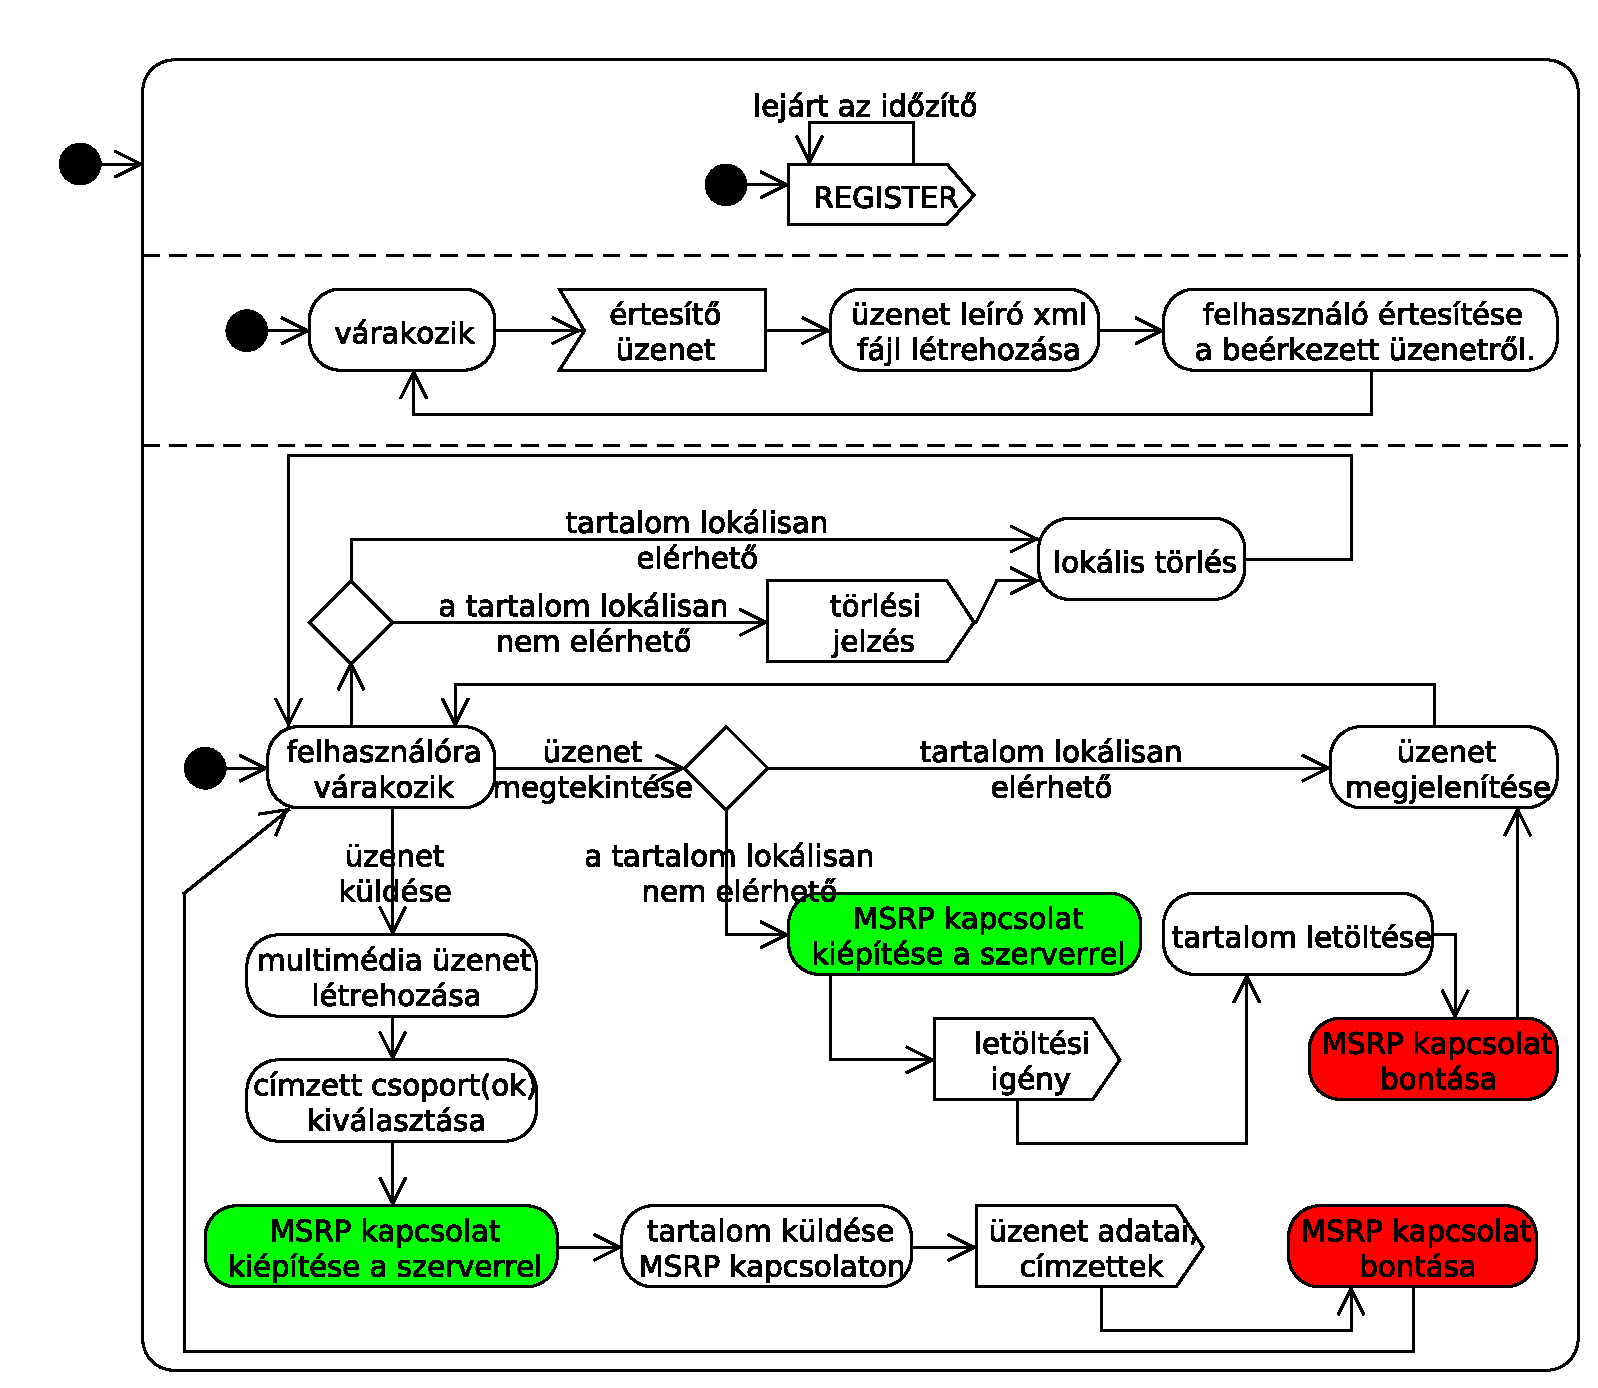
\includegraphics{img/client_statemachine_full.eps}}
\caption{A kliens állapotdiagramja}
\label{fig:client_statemachine_full}
\end{figure}

Az alkalmazás grafikus felületen fogadja a felhasználó által végrahajtott akciókat. A felhasználó kétféle tevékenységet végezhet. Egyrészt a már elküldött vagy beérkezett vagy multimédia üzeneteket szeretné megtekinteni, másrészt egy új multimédia üzenetet szeretne küldeni a felhasználók egy csoportjának. 

Az elküldött üzenetek megtekintése egyszerűen a kiválasztott üzenet adatainak megjelenítése egy grafikus ablakban, lehetőséget adva a multimédia tartalom lejátszására, megtekintésére. Az elküldött üzeneteknél a kliens oldalon minden adat rendelkezésre áll, beleértve a multimédia üzenet tényleges tartalmát.

A beérkező üzenetek esetében a multimédia tartalom kliens oldalon vagy rendelkezésre áll, vagy nem. Utóbbi eset -- azaz, hogy a tartalom lokálisan nem elérhető -- azt jelenti, hogy a szerver a multimédia üzenetről küldött értesítő MESSAGE kérését a kliens sikeresen feldolgozta, de a multimédia tartalmat még nem töltötte le a szervertől. Ilyenkor a kliensnek a tartalom megtekintéséhez ki kell építenie egy MSRP kapcsolatot a szerver oldallal, a kapcsolaton a multimédia tartalmat letölteni, majd bontani a kapcsolatot. A kliens az MSRP kapcsolat felépítése után a letölteni kívánt tartalom azonosítóját egy MESSAGE kérésben\footnotemark[2] (típusa DOWNLOAD\_CONTENT) küldi el a szervernek. A letöltés befejeződése után megjeleníthető a multimédia üzenet. \Aref{fig:client_statemachine_full}.~ábrán az MSRP kapcsolat felépítésének (zöld állapot), valamint bontásának (piros állapot) folyamata egy összetett állapot, amelyeket a később, \aref{fig:create_and_destroy_msrp_connection}.~ábrán részletesen bemutatok.

A felhasználó törölheti multimédia üzeneteket. Abban az esetben, ha egy multimédia üzenet minden része lokálisan elérhető, úgy egyszerűen törölheti az üzenetet. Amikor a multimédia tartalom nem elérhető, azaz még nem került átvitelre a szerver és a kliens között, úgy egy MESSAGE kérésben (típusa DELETE\_MESSAGE) értesíteni kell a szerver oldalt a lokálisan letörölt üzenetekről. Utóbbi azért szükséges, hogy a szerver ,,törölt'' állapotra állíthassa az üzenethez tartozó felhasználói bejegyzés értesítési státuszát. 
 
Végül a felhasználó multimédia üzenetet küldhet egy kiválasztott csoportnak. Az üzenet tartalma kétféle forrásból származhat. A kliens vagy fájlrendszeren már meglévő multimédia tartalmat választ ki, vagy a számítógéphez csatlakozó audiovizuális eszközök segítségével hozza létre azt. Miután a tartalom rendelkezésre áll, kiválasztja a címzett csoportot, kitölti az üzenet tárgyát, majd elküldi a szervernek a teljes multimédia üzenetet. A küldés folyamata azzal kezdődik, hogy a kliens felépít egy MSRP kapcsolatot a szerverrel. A multimédia tartalmat a felépített kapcsolaton elküldi a szervernek. A tartalom sikeres küldése után az üzenet címzettjeit, tárgyát, egyéb információit egy SIP MESSAGE kérés törzsében, XML formában szintén elküldi a szerver oldalnak. A MESSAGE kérés típusa MESSAGE\_DATA. Miután a MESSAGE kérést is sikeresen elküldte, bontja az MSRP kapcsolatot a szerverrel. A multimédia üzenetküldés folyamata ezzel befejeződött.

\medskip
Nézzük meg, a kliens hogyan építi fel az MSRP kapcsolatot a szerverrel. Az MSRP kapcsolat felépítésének folyamatát \aref{fig:create_msrp_connection}.~ábrán követhetjük nyomon. A kliens első lépésként létrehoz egy lokális TCP socket-et, amelyen majd az MSRP csomagok fogadása történik. Miután az említett socket egy szabad porton létrejött, a kliens generál egy egyedi MSRP kapcsolat azonosítót. A TCP socket címe és portja, valamint az MSRP azonosító együttesen egyértelműen meghatároz egy MSRP kapcsolatot. A kliens a következő lépésként a TCP socket adataiból, valamint az MSRP azonosítóból létrehoz egy SDP leírót, amit egy SIP INVITE kérés törzsében elküld a szervernek. A szerver az INVITE hatására szintén generál egy SDP leírót, amit egy 200 OK SIP válaszban elküld a kliensnek. A kliens a beérkező válaszban található szerver oldali SDP leíró alapján létrehoz egy, az MSRP csomagok küldését végző TCP kapcsolatot. Utóbbi kapcsolat a szerver oldali fogadó TCP socket-hez fog kapcsolódni. A kapcsolat felépítési folyamat befejezéseként a kliens létrehozza az MSRP kapcsolatot, majd SIP ACK nyugtát küld a szervernek, jelezvén, hogy készen áll az MSRP kapcsolaton való adatátvitelre.

\begin{figure}[htbp]
  \begin{center}
    \subfloat[A kapcsolat felépítése]{\label{fig:create_msrp_connection}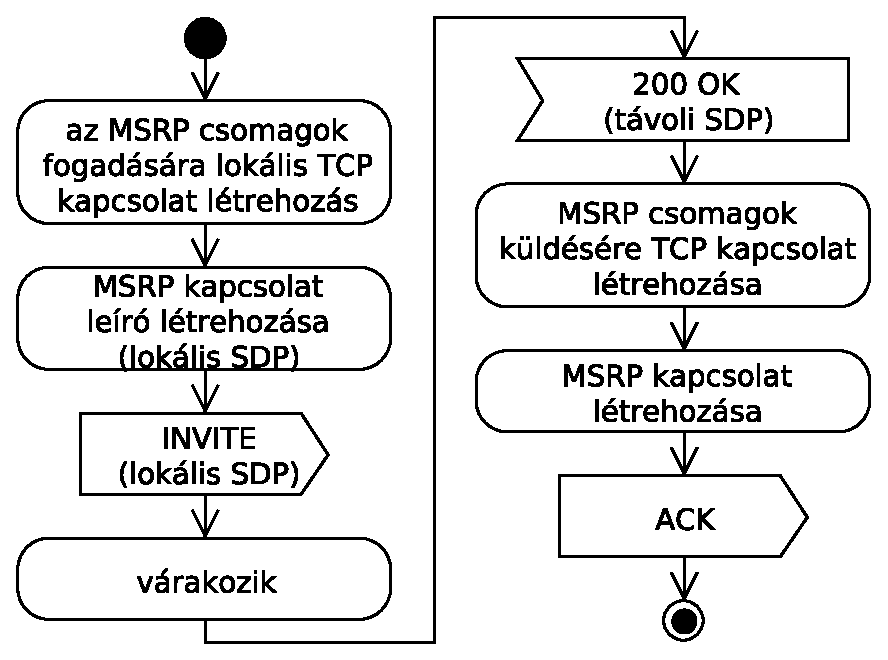
\includegraphics[scale=0.47]{img/client_create_msrp_connecton.eps}}
    \hspace{0.2in}
    \subfloat[A kapcsolat bontása]{\label{fig:destroy_msrp_connection}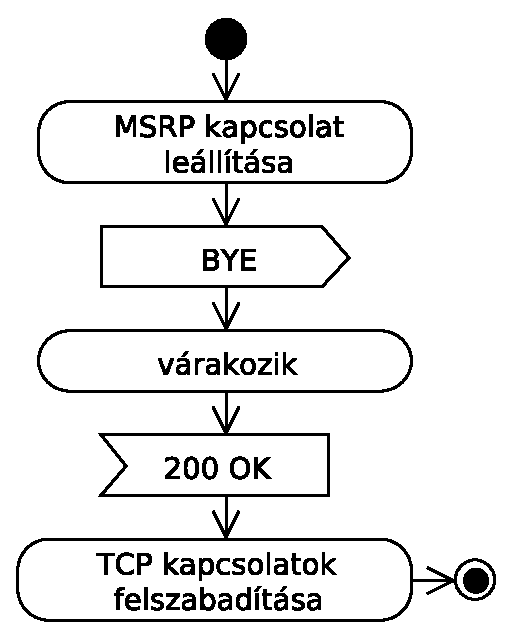
\includegraphics[scale=0.47]{img/client_destroy_msrp_connecton.eps}}
  \end{center}
  \caption{Az MSRP kapcsolat felépítése és bontása}
  \label{fig:create_and_destroy_msrp_connection}
\end{figure}

Az MSRP kapcsolat bontásának folyamata \aref{fig:destroy_msrp_connection}.~ábrán látható. Miután az MSRP kapcsolaton minden adat sikeresen átment, a kliens SIP BYE üzenetet küld a szervernek, ezzel jelezvén, hogy a felépített MSRP kapcsolat bontható. A szerver 200~OK válasz küldésével nyugtázza a kapcsolat bontását. A kliens a 200-as válasz hatására felszabadítja az MSRP kapcsolathoz használt erőforrásokat.

\subsubsection{A szerver megvalósítása}
\label{sec:szervermegvalositas}

A szerver állapotgépe \aref{fig:server_statemachine_full}.~ábrán látható. A szerver folyamatosan várja a kliensek által küldött SIP üzeneteket. A beérkező üzenetnek többféle akciót hajthat végre.

A szerver beérkező SIP REGISTER kérés esetén megnézi, hogy a küldő felhasználó szerepel-e az elérhető felhasználók listájában. Ha a felhasználó nem szerepel benne, akkor a szerver hozzáadja őt a listához. Ezután megnézi, hogy az adott felhasználónak vannak-e új üzenetei, találat esetén létrehoz egy értesítő MESSAGE üzenetet a beérkezett új üzenetek adataiból, és elküldi azt a felhasználónak. Utolsó lépésként elindítja a felhasználóhoz tartozó, REGISTER üzenet lejárati idejével inicializált időzítőt. Abban az esetben, amikor a REGISTER-t küldő felhasználó már szerepel az elérhető felhasználók listájában, akkor csak az utolsó lépés, azaz az időzítő újraindítása történik.

INVITE kérés vétele azt jelenti, hogy a küldő kliens MSRP kapcsolatot kíván felépíteni a szerverrel. Ilyenkor a szerver megvizsgálja, hogy létezik-e már az MSRP kapcsolatokon érkező csomagok fogadására létrehozott TCP socket (fogadó socket). Amennyiben létezik ilyen socket, a szerver a socket jellemzői (IP cím és port) alapján generál egy MSRP kapcsolatot leíró SDP leírót. Utóbbi leíró a szerver szemszögéből jellemzi a létrehozandó MSRP kapcsolatot. Abban az esetben, ha a szerver oldalán nem létezik fogadó socket, akkor létrehoz egyet, majd ezután generálja le a kapcsolatot leíró SDP információkat.  Az INVITE üzenet törzsében található a felépítendő MSRP kapcsolat kliens oldalát jellemző SDP leíró információk (kliens oldali fogadó TCP kapcsolat IP cím, port, MSRP kapcsolat azonosító) . Az INVITE törzsében megtalálható leíró információk alapján a szerver létrehoz egy, az MSRP csomagok küldését megvalósító TCP socketet (küldő socket). Utóbbi socket majd a kliens oldali fogadó TCP sockethez kapcsolódik, a szerver ezen a socketen küldi a kliens felé létrehozott MSRP kapcsolaton az MSRP csomagokat. A folyamat végén a szerver egy 200OK típusú SIP válasz törzsében elküldi az MSRP kapcsolatot szerver oldaláról leíró SDP információkat a kliensnek.

A szerverhez beérkező SIP ACK üzenet azt jelenti, hogy az előző bekezdésben leírt, INVITE-ra küldött 200OK üzenetet a kliens oldal sikeresen megkapta, és ő is létrehozott egy MSRP csomagok küldését végző TCP socketet, illetve létrehozta az MSRP kapcsolatot. Az MSRP kapcsolat létrehozásának folyamatában még annyi hátravan, hogy a szerver oldalon létrehozott küldő TCP socket ténylegesen kapcsolódjon a kliens oldali fogadó TCP socket-hez, majd az MSRP kapcsolat a szerver oldalán is létrejöjjön. Ennek eredményeként befejeződik a kliens és a szerver közötti MSRP kapcsolat kiépítése. Ezen az MSRP kapcsolaton a multimédia üzenethez kapcsolódó tartalom kerül majd átvitelre.

Miután egy kliens és a szerver között fennálló MSRP kapcsolaton a multimédia üzenet teljes tartalma átvitelre került, az MSRP kapcsolatra már nincs szükség. Ilyenkor a kliens SIP BYE kérést küld a szervernek, ezzel kezdeményezve az MSRP kapcsolat bontását. A szerver a kérés hatására bontja az MSRP  kapcsolatot, felszabadítja a klienssel létrehozott TCP kapcsolatok erőforrásait, majd 200OK válaszban nyugtázza a kliens felé, hogy a kapcsolat bontás sikeres volt.

\begin{figure}[htbp]
\center
\resizebox{14cm}{!}{
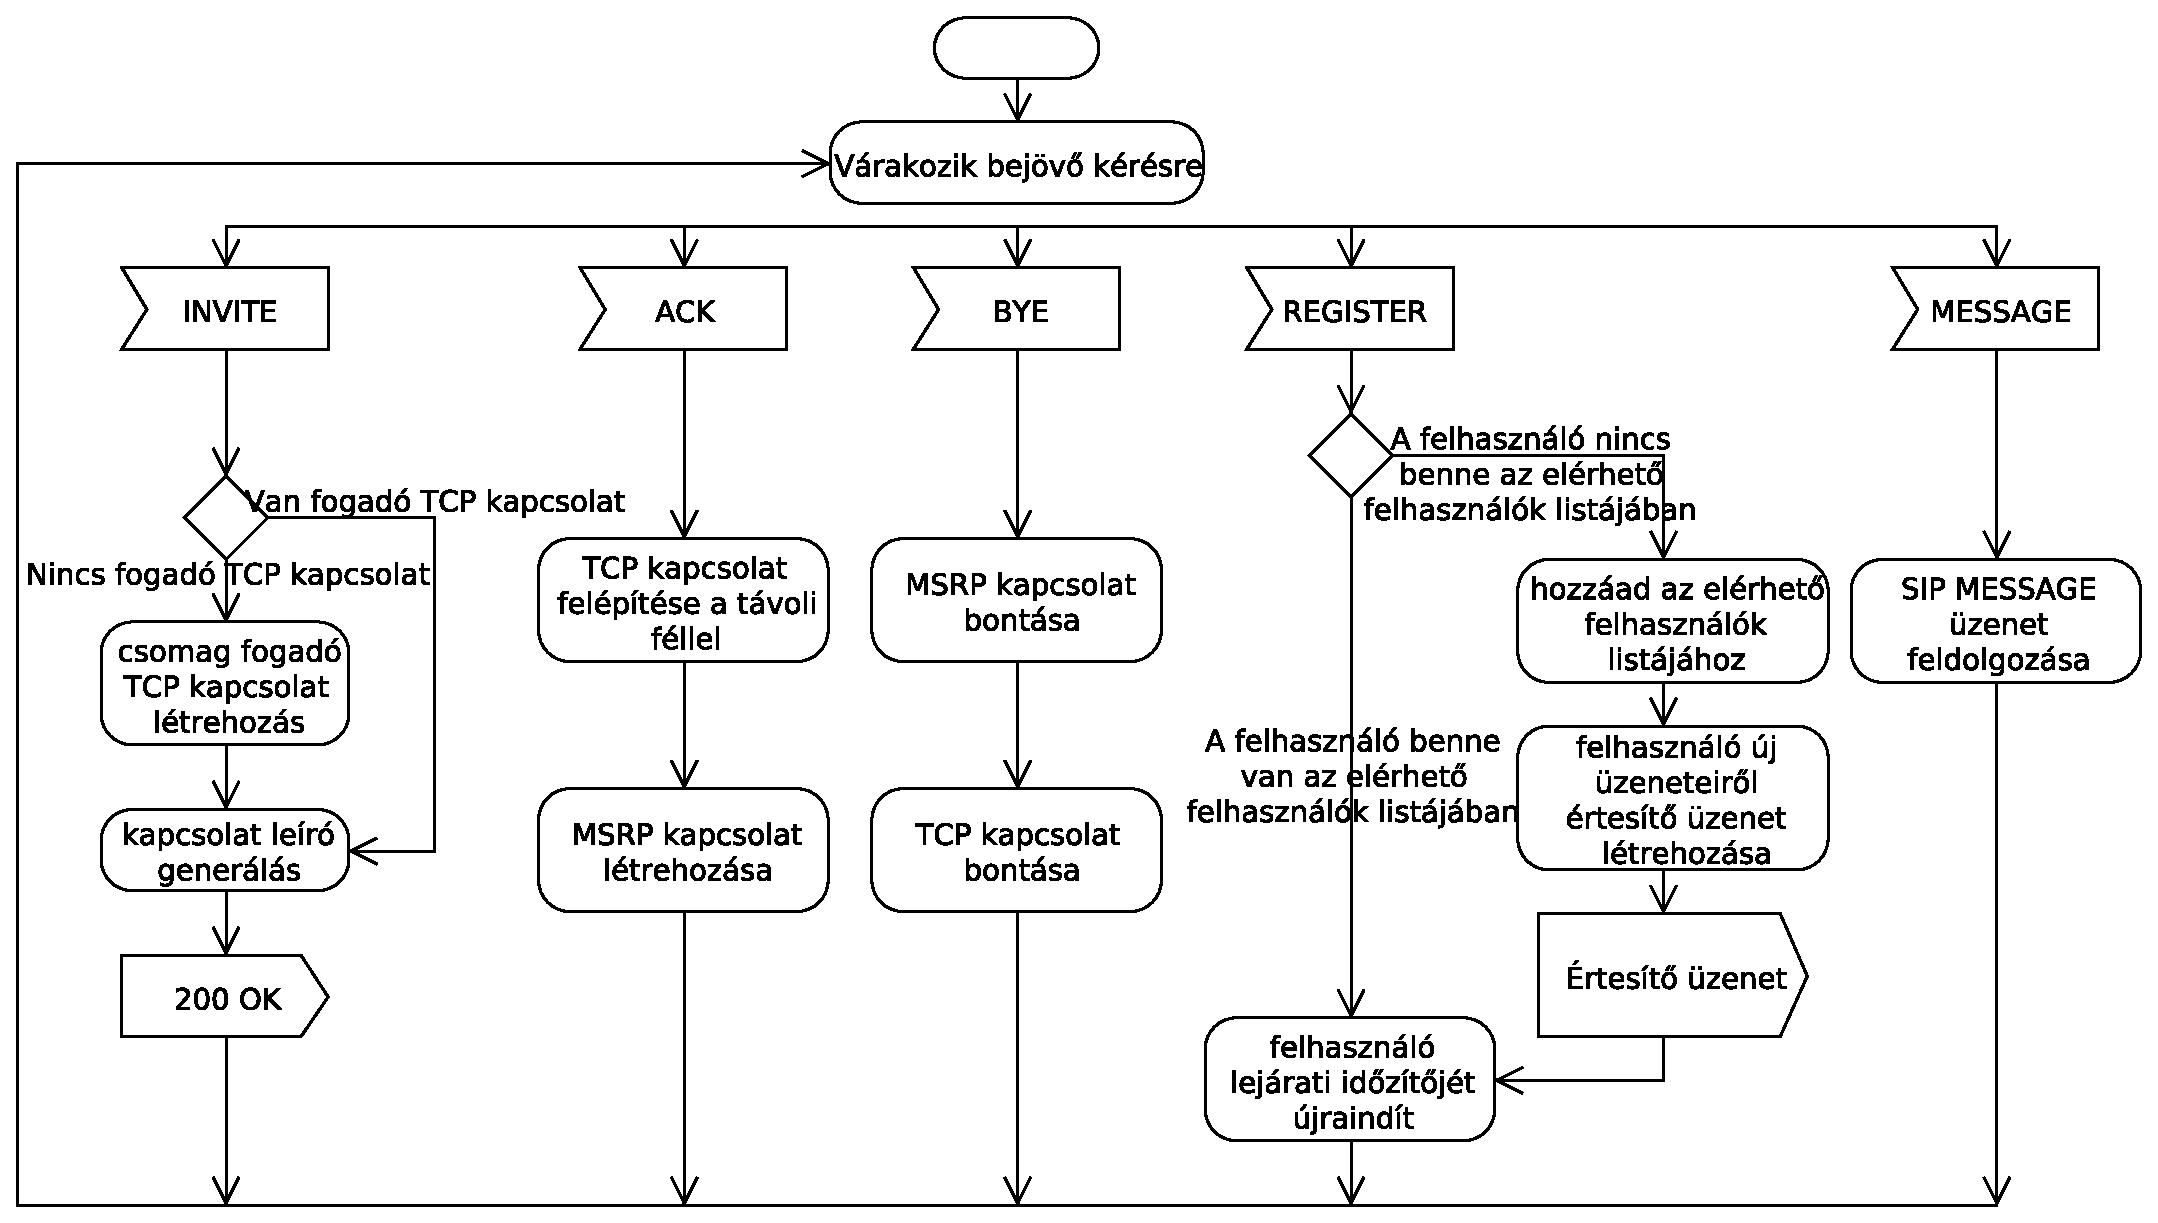
\includegraphics{img/server_statemachine_full.eps}}
\caption{A szerver állapotgépe}
\label{fig:server_statemachine_full}
\end{figure}

A szerver a kliensek felől fogadhat SIP MESSAGE kéréseket, amelyek határása többféle akciót hajthat végre. \Aref{fig:server_statemachine_full}.~ábra bal oldalán található, szürke állapot egy összetett állapot, amelyben a vett SIP MESSAGE törzsében lévő tartalom a szerver oldalon más-más tevékenységet vált ki. Az állapot részletezése \aref{fig:server_statemachine_message}.~ábrán látható.

\begin{figure}[htbp]
\center
\resizebox{12cm}{!}{
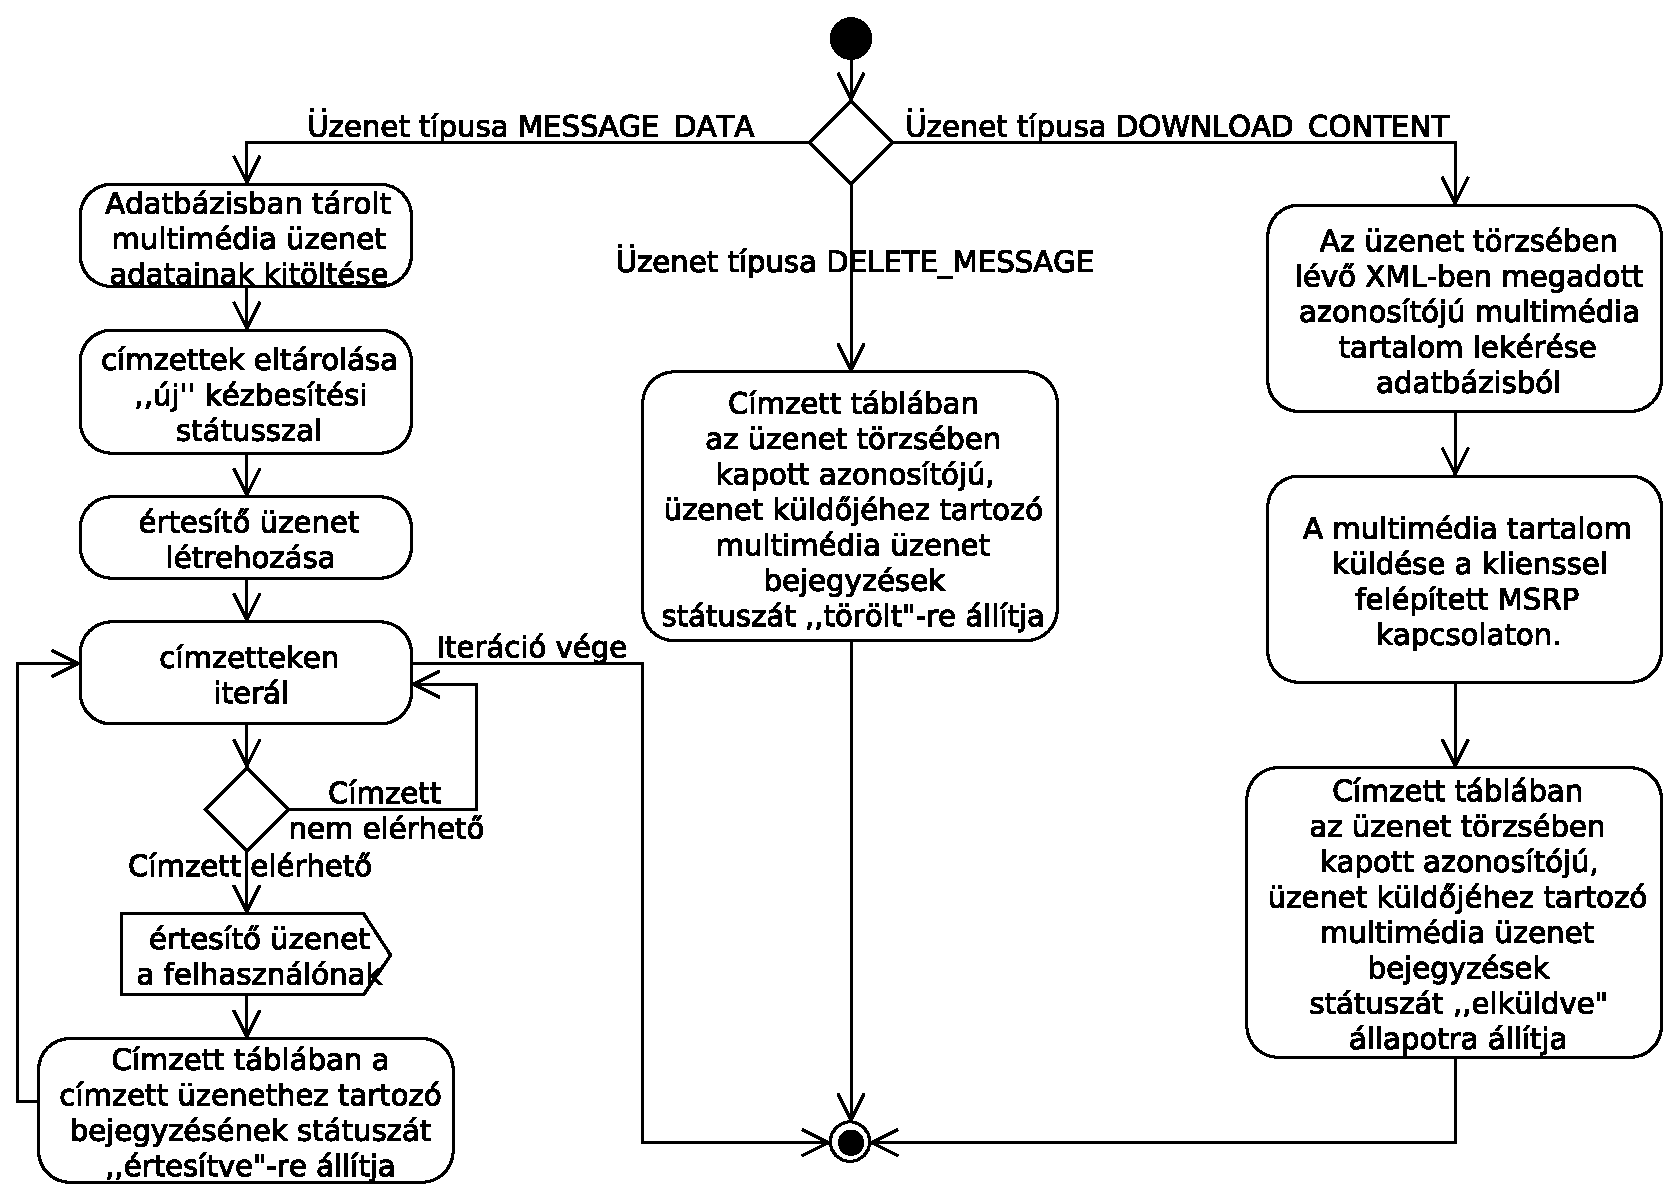
\includegraphics{img/server_statemachine_message.eps}}
\caption{A szerver állapotgépe}
\label{fig:server_statemachine_message}
\end{figure}

Az üzenetküldő szolgáltatásban használt SIP MESSAGE kérések törzsének tartalma \aref{sec:sip_message}.~részben leírt adatokat tartalmazhatja.

A multimédia üzenet küldésének folyamatában az első lépés az üzenethez tartozó tartalom a kliens és a szerver közötti MSRP kapcsolaton történő átvitele. Miután a tartalom küldése sikeresen megtörtént, a kliensnek az üzenethez tartozó egyéb információkat is el kell küldenie a szervernek. A kliens az adatokat egy SIP MESSAGE kérés törzsében, XML formában küldi el a szervernek. Ilyen információk pl. a címzettek listája, az üzenet tárgya, stb. Az XML tartalmazza a kapcsolódó multimédia tartalom MSRP átvitel során használt egyedi azonosítóját is, így az XML-ben kapott adatok egyértelműen köthetőek a már eltárolt multimédia tartalomhoz.  Az XMLből kinyerhető a MESSAGE kérés típusa is, amely ez esetben MESSAGE\_DATA. A szerver a kérés vétele után a már adatbázisban (messages táblában) eltárolt multimédia tartalomhoz kitölti a többi mező értékét, mint a küldő neve és SIP URI-ja, az üzenet tárgya, a multimédia tartalom típusa, stb. Az XML tartalmazza a címzetteket is, őket is beszúrja a címzetteket tároló adatbázis táblába (recipients). Miután az adatok eltárolása sikeresen megtörtént, a szerver létrehoz az új üzenetből egy értesítő MESSAGE kérést, amelynek törzsébe XML formában elhelyezi az új multimédia üzenetet leíró adatokat (üzenet azonosítója, feladó adatai, multimédia tartalom típusa, stb.). Az utóbbi kérés típusának NOTIFY\_USER-t állít be. Az így létrehozott MESSAGE kérést a multimédia üzenet minden elérhető címzettjének elküldi, majd a címzett táblában az értesített felhasználó multimédia üzenethez tartozó bejegyzésének értesítési státuszát ,,értesítve'' állapotra állítja. Utóbbi lépés azért szükséges, hogy a szerver tisztában legyen azzal, melyik üzenetről küldött már értesítést az adott címzettnek, és melyikről még nem.

Ha egy kliens meg szeretné tekinteni az üzenet tartalmát, akkor DOWNLOAD\_CONTENT típusú MESSAGE kérést hoz létre, amelynek törzse tartalmazza a letölteni kívánt multimédia üzenet azonosítóját. Amikor a szerver egy ilyen típusú kérést vesz, adatbázisból kinyeri a multimédia üzenet tartalmát, majd a klienssel előzetesen kiépített MSRP kapcsolaton elküldi a kért tartalmat a kliensnek. Sikeres küldés után a multimédia üzenethez tartozó, az adott címzett adatbázis bejegyzésének kézbesítési státuszát ,,elküldve'' állapotra állítja.

Amennyiben a szerver egy klienstől DELETE\_MESSAGE típusú SIP MESSAGE kérés kap, annak törzsében lévő XML-ben megtalálható azonosítójú üzenethez tartozó felhasználói bejegyzés kézbesítési státuszát ,,törölt''-re állítja az adatbázisban.  


\subsection{Összefoglalás}

